%%
%% This is file `esapub.tex',
%% generated with the docstrip utility.
%%
%% The original source files were:
%%
%% esapub.dtx  (with options: `manual')
%% ============================================
%% This is the manual describing the usage of
%%      esapub.cls
%% ============================================
%% Copyright 1999 Patrick W Daly
%% Max-Planck-Institut f\"ur Aeronomie
%% Max-Planck-Str. 2
%% D-37191 Katlenburg-Lindau
%% Germany
%% E-mail: daly@linmpi.mpg.de
%%
%% -------------------------------------------------
\documentclass[a4paper,twocolumn]{spaceDebrisC} % European paper
\pagestyle{empty}

\bibliographystyle{plain}

\usepackage{float}

\usepackage{url} % Ensure URLs are properly formatted
\usepackage{xcolor}

% \pagecolor[rgb]{0.0,0.0,0.0}
% \color[rgb]{1,1,1}

\usepackage[section]{placeins} % ensures that floats are placed in their section
\makeatletter
\AtBeginDocument{%
  \expandafter\renewcommand\expandafter\subsection\expandafter{%
    \expandafter\FloatBarrier\subsection
 }%
}
\makeatother

% \makeatletter
% \AtBeginDocument{%
%   \expandafter\renewcommand\expandafter\subsubsection\expandafter{%
%     \expandafter\FloatBarrier\subsubsection
%   }%
% }
% \makeatother

\usepackage{colortbl}
\usepackage{booktabs}
\usepackage{subcaption}
\usepackage{times}
\usepackage[numbers]{natbib}
\usepackage{graphicx}
\usepackage{bm} % for bold math
\usepackage{mathtools} % for \prescript
\usepackage{amssymb}
\usepackage{amsfonts}
\usepackage{adjustbox}

\newcommand{\grule}[0]{\arrayrulecolor{darkgray}\cmidrule(){1-2}}
\newcommand{\brule}[0]{\arrayrulecolor{black} \bottomrule}

\newcommand{\vctr}[1]{\bm{#1}}
\newcommand{\unitv}[1]{\hat{\vctr{#1}}}
\newcommand{\preup}[1]{\prescript{#1}{}{}}
\newcommand{\rf}[1]{\mathcal{\MakeUppercase{#1}}}
\newcommand{\dcm}[1]{\left[\rf{#1}\right]}
\newcommand{\vrf}[2]{\preup{\rf{#1}}\vctr{#2}}
\newcommand{\mbar}[0]{\;\middle|\;}
\newcommand{\prf}[1]{\preup{\rf{#1}}}
\newcommand{\norm}[1]{\left\lVert#1\right\rVert}

\newcommand{\matcp}[1]{\left[#1 \times\right]}
\newcommand{\rthree}[0]{$\mathbb{R}^3$\:}
\newcommand{\sthree}[0]{$\mathbb{S}^3$\:}
\newcommand{\sothree}[0]{$SO_3$}

\newcommand{\figbig}[0]{0.5\textwidth}
\newcommand{\figmed}[0]{0.4\textwidth}
\newcommand{\figsmall}[0]{0.3\textwidth}

\newcommand{\subfigmed}[0]{0.4\textwidth}
\newcommand{\subfigsm}[0]{0.29\textwidth}
\newcommand{\subfigbig}[0]{0.43\textwidth}

\DeclareMathOperator{\atantwo}{atan2}
\DeclareMathOperator{\fl}{floor}
\DeclareMathOperator*{\argmin}{arg\,min}

\title{Optimal Light Curve Attitude Inversion with Measurement Noise: Two Case Studies}
\author{Liam Robinson}
\author{Carolin Frueh}
\affil{Purdue University, West Lafayette, United States, Email: \texttt{\{robin502, cfrueh\}$@$purdue.edu}}

\begin{document}

\keywords{Light curve inversion; Atitude estimation; Photometry; Inverse problems}

\maketitle

\begin{abstract}

Understanding the orientation and angular velocity state of active or passive human-made space objects is critical for many space situational awareness operations like long-term orbit propagation, anomaly resolution, determining mission status, and active debris removal. Beyond low-Earth orbit, optical telescopes are predominantly used to track space objects. Due to atmospheric distortion and aperture size, it is generally impossible to resolve even large satellites and rocket bodies in optical ground-based imagery. As a result, shape and orientation information is unavailable in individual images, but a measurement of the object's total brightness can still be obtained. Even if the object's shape and reflective properties are known, any given brightness measurement will generally correspond to infinitely many possible orientations. To constrain the solution space, the brightness can be tracked over time -- producing a sequence of measurements called a light curve. If the object's identity is known, its attitude profile can be estimated from the light curve -- up to certain ambiguities -- through a process known as light curve attitude inversion. Due to symmetries in the observation geometry and object shape, there may be multiple attitude profiles that are equally likely to produce any given light curve. Environmental and instrumental measurement noise worsens these ambiguities. To reliably identify these ambiguous solutions, global attitude inversion methods must thoroughly search the solution space.

In this work, we apply a BFGS-based multi-start global attitude inversion algorithm to efficiently solve the attitude inversion problem globally. Results for synthetic observations are presented for a generic upper stage. Results for real observations taken by the Purdue Optical Ground Station of Delta I upper stage and the ECHOSTAR II satellite are also presented. Given a light curve with an estimate of the shape and reflective properties of the object, our procedure searches the space of initial orientations, angular velocities, and inertia tensors to find initial conditions that produce light curves with low error compared to the observed values. Our formulation inherently accounts for the aforementioned ambiguities, the physical constraints of torque-free rigid body motion, and the noise in the light curve.

\end{abstract}

\section{Introduction}

Knowledge of spacecraft orientation and angular velocity states is critical for many space situational awareness (SSA) tasks. Understanding the evolution of high area-to-mass ratio objects \cite{frueh2014} and decommissioned satellites \cite{rachman2023}, planning and executing active debris removal \cite{bonnal2013}, and recovering from mission anomalies \cite{umansky2023} all require attitude information. 

Methods for estimating the attitude state of uncontrolled space objects from light curves differ significantly depending on the presence of an initial guess. If prior knowledge is available, many filter-based approaches have been developed to process new photometry to update the guess orientation and angular velocity. This class of methods includes single Kalman filters \cite{burton2021two, gagnon2024, wetterer2009}, and multi-filter multiple-model adaptive estimation (MMAE) schemes \cite{linares2014space, dianetti2020}. These approaches can be very effective if the initial state estimate is close to the truth, but have been reported to diverge even in cases when the initial guess is within $5^\circ$ of the ground truth orientation and $0.03^\circ/s^{-1}$ in angular velocity error \cite{gagnon2024} due to measurement nonlinearity and ambiguities.

If no initial attitude guess is available, as in most cases of passive debris observation, the inversion problem must be solved globally. Filtering approaches can be applied here too; particle \cite{linares2014particle, holzinger2014} and Bayesian Multi-Hypothesis filters \cite{burton2021two, cabrera2023} have shown promise in prior work, but still rely on high-quality priors as with the single-hypothesis Kalman filters. In the absence of any prior knowledge about the object's attitude state, simulated annealing \cite{gagnon2024, clark2020}, genetic algorithms \cite{gagnon2024, piergentili2017, clark2020}, and particle swarm optimizers (PSOs) \cite{clark2020, clark2022, burton2024journal, burton2024scitech, gagnon2024, gagnon2025} can be applied to search the solution space exhaustively.

While much work has performed full state attitude inversion on simulated light curve data \cite{burton2024journal, gagnon2024, robinson2025att}, studies using real data often focus on estimating an assumed constant spin rate and axis of rotation for the observed object. These assumptions simplifies the estimation process, but can lead to misleading conclusions when the observed object has a complex rotation state.

Frequency analysis in the form of periodograms, Fourier transforms, or epoch folding, is often used to determine the spin rate based on the light curve's frequency spectrum \cite{silha2015, silha2021, isoletta2024, schildknecht2015, pittet2017, yanagisawa2012, koshkin2018}. If optical material properties are known, the width of a single specular glint can provide sufficient information to determine the rotation rate \cite{hinks2016}. There has also been interest in tracking the evolution of spin rates over time for different classes of objects in different orbital regimes \cite{koshkin2018, blacketer2022, karpov2016}. These spin rate determination methods are designed for single-axis rotations and can fail for tumbling objects.

The rotation axis is often estimated for diffusely reflecting objects that are well-approximated as ellipsoids via the so-called amplitude method \cite{williams1979location} which has been extended for combined spin and precession motion \cite{yanagisawa2012}. For light curves with strong specular peaks, the timing of these glints can be used to determine the constant rotation axis given multiple passes of observations \cite{vananti2023, koshkin2018}. These approaches are not applicable for generalized rigid body motion where no simplifying assumptions about the location of the spin axis are available.

The simplifying assumptions of constant, single-axis rotation that are commonly made when working with real data enable elegant solutions, but break down when the observed object is in a complex spin profile. Methods for full attitude state solutions -- time-varying orientation and angular velocities -- have been developed \cite{clark2022, burton2024journal, gagnon2024, linares2014particle}, but are seldom applied to real data. Works that have been successful at estimating a full rigid body attitude state from real data include genetic algorithms \cite{piergentili2020, gallucci2020} and brute-force grid search \cite{shafer2017}. Any full-state estimation method must tackle the inherent computational complexity, lack of knowledge of material reflectivities, and the presence of measurement noise.

In this paper, we describe a global full-state attitude solver inspired by recent PSO work \cite{burton2024journal} but is easier to tune, can be fully parallelized, and is robust to significant measurement noise \cite{robinson2025att}. Further, our method differs from other global estimation methods in that we do not seek to find one optimal solution and instead search for a collection of high-quality local minima to directly study the many ambiguous solutions for a given light curve. Our approach is designed specifically for use with real data as we take time-varying measurement noise and uncertainties in the body moments of inertia into account explicitly. 

To solve the optimization problem, we sample many candidate solutions scattered throughout the solution space and perform gradient-based optimization on each using the BFGS algorithm. Our optimization procedure reliably converges to high-quality maximum likelihood estimates of the attitude state. The final output of our method is an array of the best solutions, ranked by their likelihood. Clusters of low-error minima can be analyzed to identify families of solutions.

This work proceeds by describing the inversion method, discussing efficient methods for computing the time-varying probability density of the light curve. We present inversion results for a simulated rocket body light curve where the ground truth is available to demonstrate the efficacy of the method, followed by results for real light curve data collected by the Purdue Optical Ground Station for a derelict ECHOSTAR satellite and Delta I rocket body. A deeper treatment of our method and additional simulated light curve results can be found in \cite{robinson2025att}.

\section{Inversion Method}

\subsection{State Definition and Dynamics}

The state vector $\vctr{x}$ is defined to be the concatenation of the Modified Rodriguez Parameter (MRP) $\vctr{p} = [p_1, p_2, p_3]^T$, the principal body frame angular velocity $\vctr{\omega} = [\omega_1, \omega_2, \omega_3]$ in radians per second, and the ratios of the principal moments of inertia $J_y / J_x$ and $J_z / J_x$ where the constant inertia tensor in principal axes is $J = \mathrm{diag}\left([J_x, J_y, J_z]\right)$:

\begin{equation}
 \vctr{x} = \begin{bmatrix} 
 p_1 & p_2 & p_3 & \omega_1 & \omega_2 & \omega_3 & J_y / J_x & J_z / J_x
  \end{bmatrix}^T.
\end{equation}

The first six elements of the state vector are time-varying with dynamics given by:

\begin{align}
 \vctr{\dot{p}} &= \frac{1}{4} \left[ \left(1 - \vctr{p} \cdot \vctr{p}\right) + 2\vctr{p} \times \vctr{\omega} + 2 \left(\vctr{\omega} \cdot \vctr{p} \right)\vctr{p} \right], \label{eq:mrp_kde} \\
 \vctr{\dot{\omega}} &= J^{-1} \left[ \left(J \vctr{\omega}\right) \times \vctr{\omega} + \vctr{M}\right]. \label{eq:rbtf_dynamics}
\end{align}

\subsection{Objective Function}

Our inversion method is based on the global minimization of a maximum-likelihood loss function which computes the negative log-likelihood of the observed light curve $\vctr{S}$ being a sample from the normal distribution defined by the estimated light curve mean $\hat{\vctr{S}}$ and the standard deviation at each $k$th timestep $\sigma_k$:

\begin{equation} \label{eq:nll_loss}
 f(\vctr{x}) = \frac{1}{m}\sum_{k=1}^{m}\left[\frac{1}{2} \ln2\pi + \ln\sigma_k + \frac{1}{2}\left(\frac{\vctr{S}_k - \hat{\vctr{S}}_k(\vctr{x})}{\sigma_k}\right)^2 \right].
 \end{equation}

Note that the constant $0.5\ln2\pi$ could be removed from the objective function, but it is retained such that $\text{exp}\left(-f(\vctr{x})\right)$ is a true likelihood. If the reflectivity of the object's faces is not well-known, we rescale the estimated light curve mean $\hat{S}(\vctr{x})$ to have equal $\ell_2$ norm to the observations to resolve the inherent albedo-area ambiguity:

\begin{equation}
 \hat{S}(\vctr{x}) = \frac{\norm{S}}{\norm{\tilde{S}(\vctr{x})}} \tilde{S}(\vctr{x}),
\end{equation}

\noindent
where $\tilde{S}(\vctr{x})$ is the original, poorly scaled, estimated light curve. In this work, the light curve and its standard deviation are always assumed to be expressed in a linear unit, e.g., analog-to-digital units (ADU) or irradiance proportional to $W/m^2$.

\subsection{Computing Local Minima} \label{sec:run_solver}

Our multi-start solution method begins by creating $n_\text{sample}$ sampled states scattered throughout the solution space -- possibly sampled from a prior distribution based on available knowledge. In the most basic case, the initial states are drawn for sample $i$ at iteration $k=0$:

\begin{equation}
 \vctr{x}_{0,i}(0) = \begin{bmatrix}\vctr{p}_{i,0}(0) \\ \vctr{\omega}_{i,0}(0) \\ \left(J_y / J_x\right)_{i,0} \\ \left(J_z / J_x\right)_{i,0}\end{bmatrix}.
\end{equation}

In this work, initial state vectors are sampled from a prior distribution, usually defined independently for the MRP, angular velocity, and inertia tensor ratios. If no information is available, as is usually the case, a uniform distribution is sampled from for the first six components of the state. In particular, $\vctr{p}_{i,0}(0)$ is uniformly randomly sampled from orientation space, $\vctr{\omega}_{i,0}(0)$ is randomly sampled from a uniform distribution of magnitudes up to $\norm{\vctr{\omega}}_\text{max}$ -- the maximum angular rate at which to initialize state samples. We determine $\norm{\vctr{\omega}}_\text{max}$ based on the maximum power positive frequency in the observed light curve $f^\star$ in Hertz and an arbitrary safety factor $f_\omega \geq 1$, selected as $f_\omega = 1.25$ for this work:

\begin{equation} \label{eq:ang_vel_max}
  \norm{\vctr{\omega}}_\text{max} = 2\pi f_\omega f^\star.
\end{equation}

Uniformly sampling over angular velocity directions, we can express the default sampling strategy for an angular velocity state as:

\begin{equation} \label{eq:omega_sampler}
  \vctr{\omega}_{i,0}(0) = \frac{m}{\sqrt{g_1^2+g_2^2+g_3^2}} \cdot \begin{bmatrix} g_1 & g_2 & g_3 \end{bmatrix}^T,
\end{equation}

\noindent
where $g_{1:3} \in \mathcal{N}(0,1)$ and $m=\mathcal{U}(c_1 \norm{\vctr{\omega}}_\text{max}, c_2 \norm{\vctr{\omega}}_\text{max})$. The constants $c_1<1$ and $c_2>1$ are chosen to correct for the fact that even for a well-chosen bound $\norm{\vctr{\omega}}_\text{max}$, there can still be numerous high-quality solutions at significantly lower or higher angular velocities that possess equal $f^\star$ values. This is a result of object shape symmetries or harmonics in spin and precession rates. We select $c_1=0.5$, $c_2=2$ for this work.

For the MRP, we first sample a quaternion $\vctr{q}_i(0) = [q_x, q_y, q_z, q_w]^T$ uniformly over orientation space:

\begin{equation}
  \vctr{q}_i(0) = \frac{1}{\sqrt{g_1^2 + g_2^2 + g_3^2 + g_4^2}} \begin{bmatrix} g_1 & g_2 & g_3 & g_4 \end{bmatrix}^T,
\end{equation}

\noindent
where $g_{1:4} \in \mathcal{N}(0,1)$, and project the quaternion into MRP space:

\begin{equation} \label{eq:mrp_sampler}
  \vctr{p}_{i,0}(0) = \frac{1}{1 + q_w} \begin{bmatrix} q_x & q_y & q_z \end{bmatrix}^T.
\end{equation}

Unlike the MRP and angular velocity, the default sampling method for inertia ratios initial samples $\left(J_y / J_x\right)_{i,0}$ and $\left(J_z / J_x\right)_{i,0}$ draws from independent, identically distributed Gaussian prior distributions with $\sigma_J$ centered at estimated values derived from the known geometry of the object $\left(J_y / J_x\right)_\text{est}$ and $\left(J_z / J_x\right)_\text{est}$, such that:

\begin{equation}
  \begin{bmatrix}
    \left(J_y / J_x\right)_{i,0} \\ \left(J_z / J_x\right)_{i,0}
  \end{bmatrix} \sim \mathcal{N} \left(\begin{bmatrix}
    \left(J_y / J_x\right)_\text{est} \\
    \left(J_z / J_x\right)_\text{est} \end{bmatrix}, \sigma_J I_2 \right),
\end{equation}

\noindent
where $I_2$ is the $2\times2$ identity matrix.

After sampling each initial state, we run the Broyden-Fletcher-Goldfarb-Shanno (BFGS) algorithm \cite{broyden1970, fletcher1970, goldfarb1970, shanno1970} to optimize each sample to a nearby local minimum $\vctr{x}_{k,i}(0)$ in the objective function such that:

\begin{equation} \label{eq:opt_problem}
 \vctr{x}_{k,i}(0) = \argmin_{\vctr{x}} f(\vctr{x}),
\end{equation}

\noindent
producing a converged initial state $\vctr{x}_{k,i}(0)$ which is a good local guess to have produced the observations. In this way, we globally search the solution space up to the density implied by $n$. Using a simpler algorithm like gradient descent can still reach convergence, but will take significantly more objective function evaluations due to the high nonlinearity of the attitude inversion problem.

In order to implement this optimization effectively without constraints, it is often necessary to take the absolute value of the intermediate inertia tensor values to maintain physical validity. 

\subsection{Classifying Candidate Solutions} \label{sec:candidate_sols}

Although all initial conditions will converge to some nearby local minimum, many of these minima will possess a low likelihood determined by $-\mathrm{exp}(f(\vctr{x}))$ where $f(\vctr{x})$ is the objective function in Equation \ref{eq:nll_loss}. As we do not generally know how large the geometric and material mismatch between the observed object and the assumed model is, we cannot put a strict bound on a likelihood level that constitutes a high-quality candidate solution. In this work, we identify candidate solutions by choosing a likelihood ratio tolerance $0 < \ell < 1$, such that all solutions $\vctr{x}_{i,k}(0)$ are candidates for the truth if:

\begin{equation} \label{eq:ell_selection_criteria}
  e^{-f\left(\vctr{x}_{i,k}(0)\right)} > \ell e^{-f\left(\vctr{x}^\star_{k}(0)\right)}.
\end{equation}

Here, $\vctr{x}^\star_{k}(0) = \argmin_{\vctr{x}_{i,k}(0)} f\left(\vctr{x}_{i,k}(0)\right) $ is the highest likelihood solution found after optimization.

\section{Computing the Light Curve}

The inversion method in this paper is not dependent on a particular approach for computing light curves and their expected standard deviations. Here, we present the models used to produce the results in Sections \ref{sec:synth_results} and \ref{sec:real_results}.

\subsection{Object Geometry Definition}

We choose to represent the surface geometry of space objects as a polyhedral mesh composed of a collection of flat facets. Each $i$th face has $n_v \geq 3$ or more vertices $\left\{ v_{i,1}, v_{i,2}, v_{i,n_v} \right\}$ and an outward-pointing normal vector $\unitv{n}_i$. The total facet area is computed for an arbitrary planar polygon via:

\begin{equation} \label{eq:poly_area}
 A(P) = \sum_{j=0}^{k-3} \frac{\| \left( \vctr{v}_{j+1} - \vctr{v}_{j} \right) \times \left( \vctr{v}_{j+2} - \vctr{v}_{j} \right)\|_2}{2}.
 \end{equation} 
 
 In any particular illumination and observation condition, a fraction of the facet's area $\tilde{a}_i$ might be Sun or observer-shadowed due to obstructing geometry before or after light reaches the surface element, respectively. The remainder of the facet's area $\bar{a}_i$ is unshadowed and contributes to the total flux reaching the observer from the object, such that the total area of each facet is $a_i = \tilde{a}_i + \bar{a}_i$. The geometry for an individual facet is displayed in Figure \ref{fig:facet_geom}.

\begin{figure}[H]
  \centering
  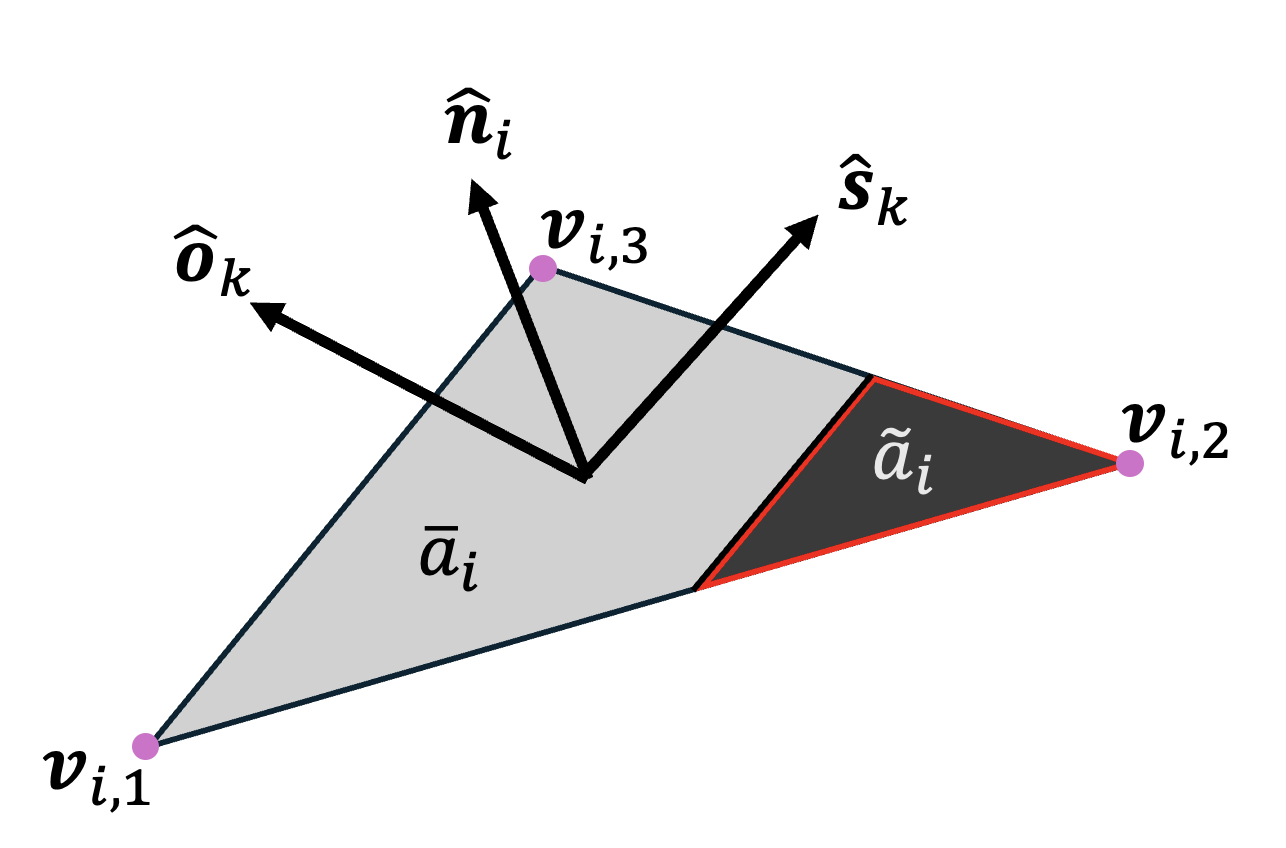
\includegraphics[width=\figmed]{obs_geom.png}
  \caption{Facet geometry including the observer direction $\unitv{o}$, Sun direction $\unitv{s}$, normal vector $\unitv{n}_i$, unshadowed area $\bar{a}_i$, shadowed area $\tilde{a}_i$, and counterclockwise vertex positions $\left\{ \vctr{v}_{i,1}, \vctr{v}_{i,2}, \vctr{v}_{i,3} \right\}$.}
  \label{fig:facet_geom}
\end{figure}

In this work, the Sun position is computed using a SPICE ephemeris kernel \cite{spice} while space object positions are propagated with SGP4 TLEs obtained from Space-Track \cite{spacetrack}.

\subsection{Computing the Unshadowed Area}

The unshadowed area $\bar{a}$ can be computed in several ways. For convex objects, $\bar{a}=a$ as self-shadowing is impossible. For highly nonconvex and detailed models composed of thousands of faces, $\bar{a}$ can be approximated on a pixel grid using shadow mapping \cite{robinson2022}. Self-shadowing can be efficiently solved semi-analytically for lower-fidelity approximations of real space object geometry by computing the mutual intersections of the polygons $P_k$ of other faces whose projections overlap with the face in question. Up to a maximum intersection depth $d$, selected for computation time, the unshadowed area can be computed via:

\begin{equation} \label{eq:us_area}
 \bar{a} = a - \sum_{d=1}^{n} \sum_{K \in \text{comb}(n,d)} (-1)^{d+1} A\left(\bigcap\limits_{k \in K} P_k\right).
\end{equation}

As the objects we investigate in this work are well-approximated with relatively simple non-convex meshes, we use the semi-analytic method to efficiently compute unshadowed areas via the Sutherland-Hodgeman algorithm \cite{sutherland1974} for each polygon intersection. Further explanation of the polygon clipping procedure for computing the total shadowed area, and accelerating this computation during inversion with the so-called shadow cache is available here \cite{robinson2025att}.

\subsection{Surface Reflectivity}

The bidirectional reflectance distribution function (BRDF) defines the amount of incident radiation from $\unitv{s}$ reflected per steradian in the observer's direction $\unitv{o}$. We choose the Blinn-Phong \cite{blinn1977} BRDF for this work as it is efficient to compute and satisfies the three main requirements for a physically meaningful BRDF as it is nonnegative, energy-conserving, and reciprocal \cite{duvenhage2013}. We avoid microfacet models for computational efficiency, and because in practice, the uncertainty in the reflective properties of the observed objects will often be larger than errors introduced by the choice of reflection model. The Blinn-Phong BRDF is parameterized by the coefficient of diffuse reflectivity $C_d$, the coefficient of specular reflectivity $C_s$, and the specular exponent $n>0$ \cite{duvenhage2013}:

\begin{equation} \label{eq:brdf_blinn_phong}
 f_r(\unitv{s}, \unitv{o}) = \frac{C_d}{\pi} + \frac{n+2}{2\pi} \frac{C_s (\unitv{n} \cdot \unitv{h})^n}{4 (\unitv{n} \cdot \unitv{s})(\unitv{n} \cdot \unitv{o})}.
\end{equation}

The coefficients of reflectivity implicity satisfy $C_a + C_s + C_d = 1$ for energy conservation, where $ 0 \leq C_a \leq 1$ is the coefficient of absorption \cite{fan2020thesis}.

Here, the halfway vector $\unitv{h}$ bisects the illumination and observation directions such that $\unitv{h} = \unitv{h} = (\unitv{s} + \unitv{o})/\norm{\unitv{s} + \unitv{o}}$ \cite{duvenhage2013}.

\subsection{Computing the Mean Observed Signal}

Given the observer $\unitv{o}_k$ and illumination directions $\unitv{s}_k$ at the $k$th observation epoch in the body frame $\mathcal{B}$, as well as the BRDF $f_{r,i}$ for each $i$th surface of the object, the fraction of incident power reflected in the direction of the observer is \cite{fan2020thesis}:

\begin{equation} \label{eq:lc_norm}
  \begin{split} 
 f_p(\unitv{s}_k, \unitv{o}_k) = \sum_{i=1}^n\prf{B}[&\bar{a}_i(\unitv{s}_k, \unitv{o}_k) f_{r,i}(\unitv{s}_k, \unitv{o}_k) \\ \cdot &(\unitv{n}_i \cdot \unitv{s}_k) (\unitv{n}_i \cdot \unitv{o}_k)]. 
  \end{split} 
\end{equation}

As many of the noise characteristics of the signal are defined in the image sensor's native unit of ADU, we use $f_p(\unitv{s}_k, \unitv{o}_k)$ to compute the light curve in ADU via:

\begin{equation} \label{eq:general_bright}
  \begin{split} 
 \bar{S}_{\text{SO},k} = &f_p(\unitv{s}_k, \unitv{o}_k) \frac{A_\circ \Delta t_k f_\odot(\vctr{r})}{g R_\oplus^2 r_k^2} \\ \cdot &\int_{0}^{\infty}{P(\lambda)Q(\lambda)T_k(\lambda) I_\odot(\lambda) \left(\frac{\lambda}{hc}\right)}\,d\lambda. 
  \end{split}
\end{equation}

Here before the integral, $A_\circ$ is the unobstructed aperture area in square meters, $\Delta t_k$ is the exposure time in seconds, $f_\odot(\vctr{r})$ is the fraction of solar irradiance reaching the space object at position $\vctr{r}$ -- accounting for the Earth's shadow, $g$ is the sensor gain in ADU per photoelectron, $R_\oplus$ is the distance from the Sun to the space object in AU, $r_k$ is the distance from the observer to the space object in kilometers. Within the integral, we account for the telescope's passband filter $P(\lambda)$, the image sensor quantum efficiency $Q(\lambda)$, the atmospheric absorption spectrum $T_k(\lambda)$, the solar irradiance spectrum $I_\odot(\lambda)$, and the inverse energy of a photon with wavelength $\lambda$, $\lambda / hc$, where $h$ is Planck's constant in Joule-seconds, and $c$ is the speed of light in vacuum in meters per second. Taken together, the integral computes the fraction of the energy reflected from the object absorbed into the image sensor, while the outer factor dimensionalizes the result to yield the mean total sensor response in ADU across all pixels due to the object's signal.

\subsection{Approximating the Measurement Noise}

This section summarizes an in-depth study of relevant noise sources in CCD and CMOS sensor light curves which can be found in \cite{robinson2025twin}.

The variance of a space object's observed brightness whose mean is determined by Equation \ref{eq:general_bright} is a combination of many independent stochastic processes. These distributions have variances $\sigma^2_\text{sensor}$ due to the sensor's integration and readout effects, $\sigma^2_\text{flat}$ from sensor flat-fielding effects, scintillation noise $\bar{S}_{\text{SO},k} \sigma^2_{Y,k}$ \cite{osborn2015}, Poisson signal shot noise $\lambda_{\text{shot},k}$, and Poisson background noise $\lambda_{\text{back},k}$. The sum of these variances yields the total signal variance in ADU:

\begin{equation} \label{eq:sigma_total}
  \begin{split}
  \sigma^2_{S,k} = &\lambda_{\text{back},k} + \bar{S}_{\text{SO},k} \sigma^2_{Y,k} + \lambda_{\text{shot},k} \\ + &\sigma^2_\text{flat} + \sigma^2_\text{sensor}.
  \end{split}
\end{equation}

The sensor noise is approximated by the independent combination of Poisson dark current $\lambda_\text{dark}$ and zero-mean Gaussian readout noise $\sigma_\text{read}^2$ \cite{krag2003}:

\begin{equation} \label{eq:sensor_noise}
  \sigma_\text{sensor}^2 = n_\text{pix} \left( \Delta t \cdot \lambda_\text{dark} + \sigma_\text{read}^2 \right).
\end{equation}

The flat field noise is modeled as a zero-mean Gaussian linearly scaling with the signal in each of the $n_\text{pix}$ pixels of the object signal $S_i$ and a constant $f_k$ fit to the sensor from flat frame observations, yielding the signal standard deviation \cite{newberry1996}: 

\begin{equation}
  \sigma_\text{flat}^2 = f_k^2 \sum_{i=1}^{n_\text{pix}} S_i^2.
\end{equation}

The background standard deviation is modeled by the sum of six independent Poisson random processes contributing to light entering the telescope optics from environmental sources. These processes and the sources of their respective models are: scattered moonlight $\lambda_{\text{moon},k}$ \cite{daniels1977}, integrated starlight $\lambda_{\text{star},k}$ \cite{krag2003}, twilight $\lambda_{\text{twi},k}$ \cite{patat2006}, zodiacal light $\lambda_{\text{zod},k}$ \cite{roach1972}, airglow $\lambda_{\text{air},k}$ \cite{krag2003}, and light pollution $\lambda_{\text{poll},k}$ \cite{falchi2016, falchi2016_data}. In summation, the total Poisson background variance is:

\begin{equation}
  \begin{split}
  \lambda_{\text{back},k} = n_{\text{pix},k} ( &\lambda_{\text{moon},k} + \lambda_{\text{star},k} + \lambda_{\text{twi},k} \\+ &\lambda_{\text{zod},k} + \lambda_{\text{air},k} + \lambda_{\text{poll},k} ).
  \end{split}
\end{equation}

The fractional scintillation noise due to atmospheric turbulence is modeled via Young's approximation \cite{osborn2015}:

\begin{equation} \label{eq:scint_noise}
  \sigma^2_{Y,k} = 10^{-6} D^{-4/3} (\Delta t)_k^{-1} \cos^{-3}\left(\gamma_k\right) e^{\frac{-2h_\text{obs}}{H}}.
\end{equation}

Here, the scintillation noise at timestep $k$ as a function of the aperture diameter $D$ in meters, the exposure time $(\Delta t)_k$ in seconds, the zenith angle $\gamma_k$, the observing station's altitude $h_\text{obs}$ in meters, and the turbulence scaleheight $H\approx8000$ meters \cite{osborn2015}.

The signal shot noise is a Poisson process as a function of the mean signal in ADU $\bar{S}_{\text{SO},k}$ and the image sensor gain $g$ in ADU per photoelectron:

\begin{equation}
  \lambda_{\text{shot},k} = \frac{\bar{S}_{\text{SO},k}}{\sqrt{g}}.
\end{equation}

After summation in Equation \ref{eq:sigma_total}, we can approximate the observed light curve as Gaussian distributed via the mean $\bar{S}_{\text{SO},k}$ from Equation \ref{eq:general_bright} and the variance $\sigma^2_{S,k}$ in $\text{ADU}^2$:

\begin{equation} \label{eq:lc_dist}
 S_{\text{SO},k} \sim \mathcal{N}\left( \bar{S}_{\text{SO},k}, \sigma^2_{S,k} \right).
 \end{equation}

\section{Attitude Inversion Results for Synthetic Data} \label{sec:synth_results}

To demonstrate the effectiveness of our inversion method, we first present results for a simulated light curve where the ground truth attitude profile is available for comparison.

\subsection{Generating the Observed Light Curve}

In order to make this simulated case realistic, we use the presented measurement noise models and introduce a mismatch between the ground truth object used to generate the measurements and the model used in inversion. The selected object is a high-fidelity model of the Saturn V second stage scaled down by a factor $10/3$ to act as a template rocket body object, shown on the right of Figure \ref{fig:rb_models}

% \begin{figure}[H]
%   \centering
%   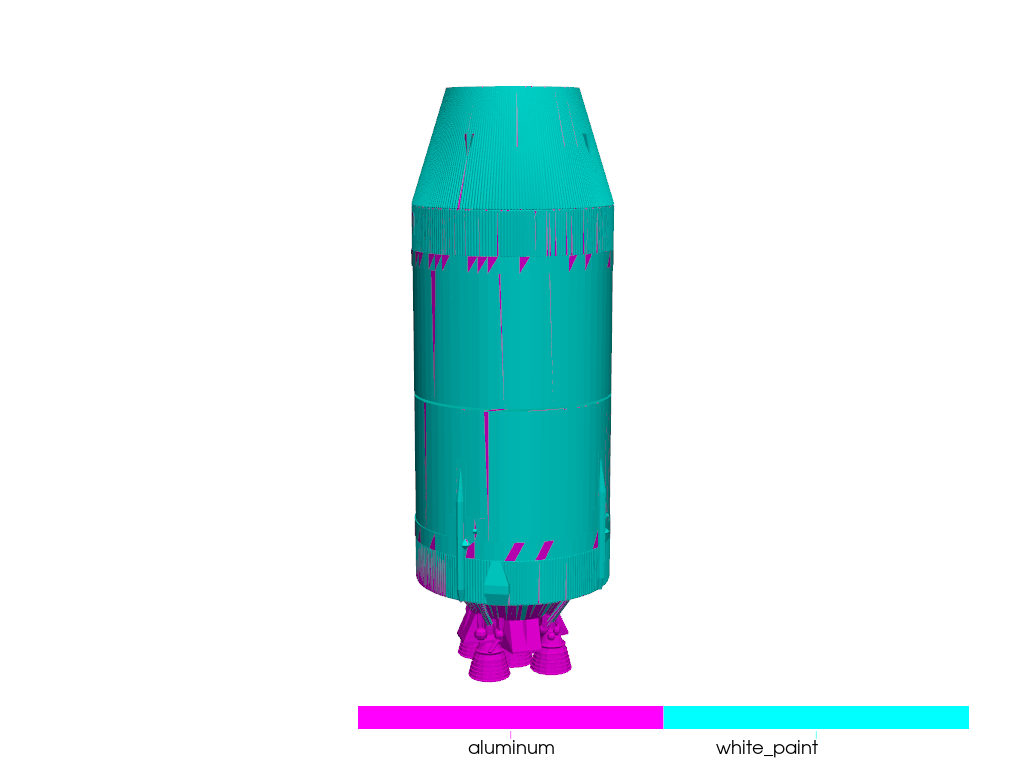
\includegraphics[width=\figsmall]{rocket_bodies2.png}
%   \caption{Simulated truth rocket body model \cite{nasa_models}.}
%   \label{fig:meas_model}
% \end{figure}

Table \ref{tb:case1_in} describes the simulated observation scenario used to produce the noisy light curve observations, placing the rocket body in the orbit of an SL-12 upper stage in geosynchronous orbit, observed by the Purdue Optical Ground Station. Relevant geographical and optical properties of this ground station are provided in the Appendix in Table \ref{tb:tele_info}. Table \ref{tb:synth_matprops} lists the material properties used in this test case.

\begin{table}[H]
  \centering
  \renewcommand{\arraystretch}{1.3} % Increase row height for better readability
  \caption{Simulated observation characteristics}
  \vspace*{6pt}
  \begin{tabular}{@{} l l @{}}
    \toprule
    Variable & Value \\ \midrule
    Target COSPAR ID & 1990-054D \\ \grule
    First obs.\ (UTC) & Mar 8, 2025 02:00:00.000 \\ \grule
    Light curve duration & $5$ minutes \\ \grule
    Observations & $100$ \\ \grule
    Integration time & $0.5$ seconds \\ \brule
  \end{tabular}
  \label{tb:case1_in}
\end{table}


\begin{table}[H]
  \centering
  \renewcommand{\arraystretch}{1.3} % Increase row height for better readability
  \caption{Reflection properties of materials used in the synthetic data test case. The white paint parameters are estimated qualitatively.}
  \vspace*{6pt}
  \begin{tabular}{@{} l l l l @{}}
    \toprule
    Material & $C_d$ & $C_s$ & $n$ \\ \midrule
    Aluminum \cite{fankhauser2023} & $0.34$ & $0.40$ & $8.9$ \\ \arrayrulecolor{darkgray}\cmidrule(){1-4}
    White paint & $0.9$ & $0.1$ & $1$ \\ \brule
  \end{tabular}
  \label{tb:synth_matprops}
\end{table}

The ground truth attitude profile and inertia tensor ratios of the simulated object are listed in Table \ref{tb:synth_att}.

\begin{table}[H]
  \centering
  \renewcommand{\arraystretch}{1.3} % Increase row height for better readability
  \caption{True object attitude profile for all test cases}
  \vspace*{6pt}
  \begin{tabular}{@{} l l @{}}
    \toprule
    Variable & Value \\ \midrule
    Initial $\vctr{p}(0)$ & $-\frac{1}{3} \begin{bmatrix} 1 & 1 & 1 \end{bmatrix}^T$ \\ \grule
    True $\vctr{\omega}(0)$ ($\text{rad}\cdot\text{s}^{-1}$) & $\vctr{\omega}(0) = \begin{bmatrix} 0.03 & 0.06 & 0.03 \end{bmatrix}^T$ \\ \grule
    Inertia tensor ratios & $J_y / J_x = 1, \: J_z / J_x = 0.25$ \\ \grule
    External torque $\vctr{M}$ & $\begin{bmatrix} 0 & 0 & 0 \end{bmatrix}^T$ \\ \brule
  \end{tabular}
  \label{tb:synth_att}
\end{table}
\FloatBarrier


Simulating the mean light curve and its approximate probability distribution via Equation \ref{eq:lc_dist} produces the light curve displayed in V-band magnitude in Figure \ref{fig:obs_mag_synth}.

% \begin{figure}[H]
%   \centering
%   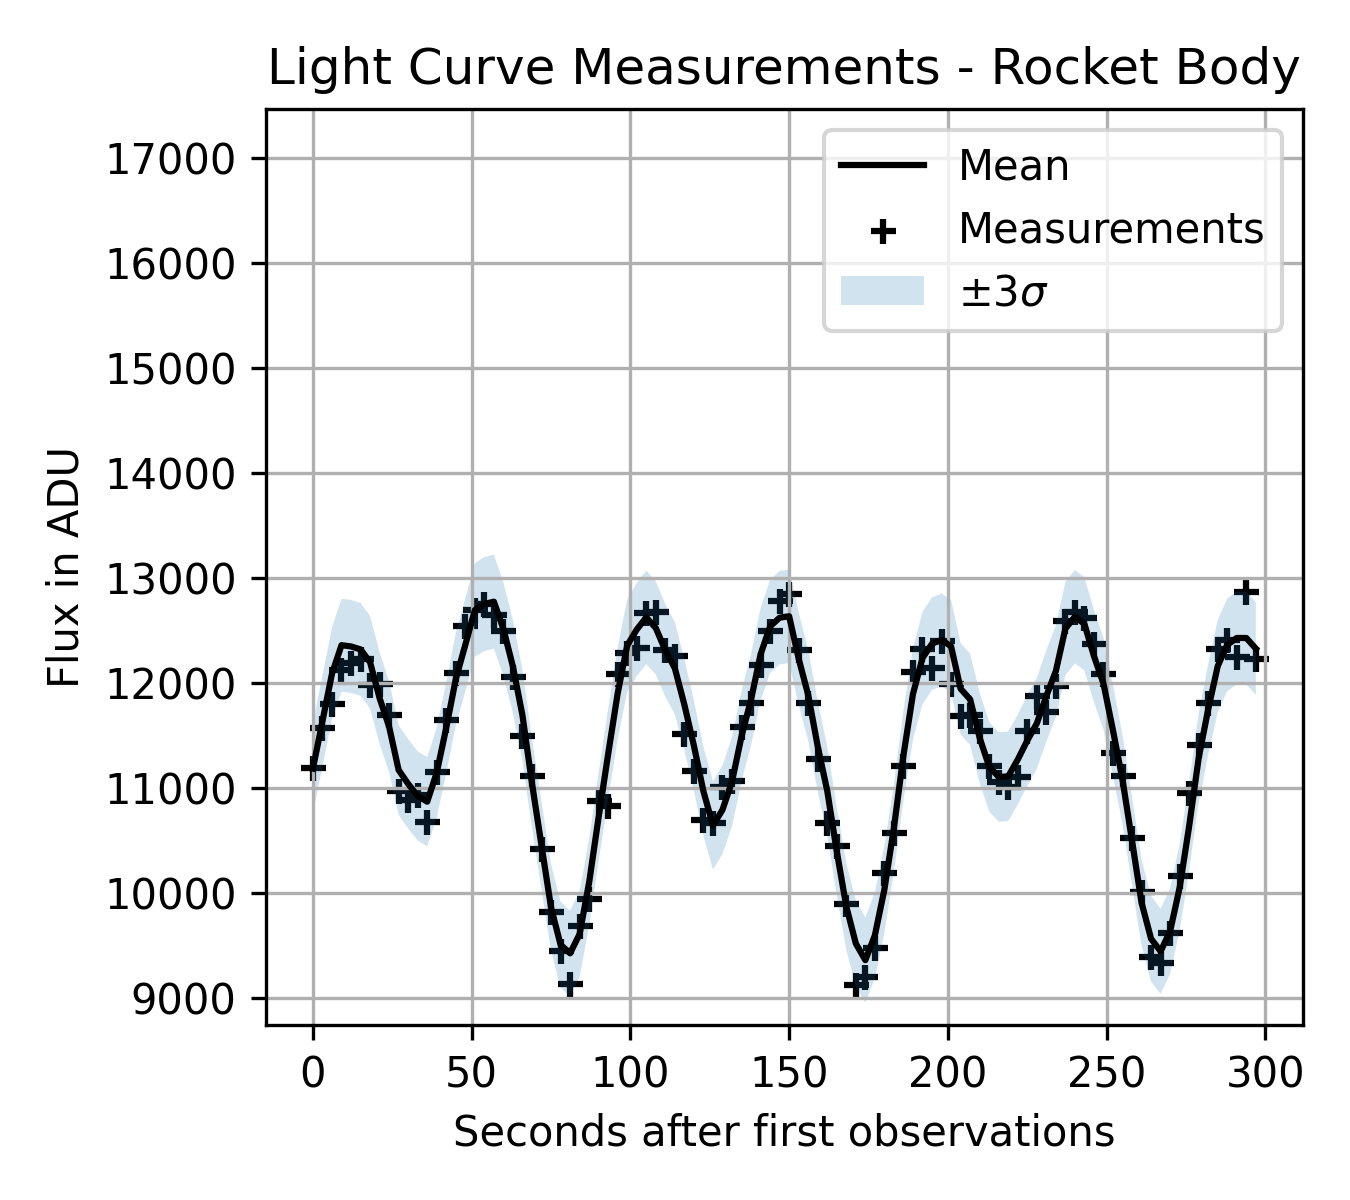
\includegraphics[width=\figmed]{light_curves_adu_rocket_body_sdc.png}
%   \caption{Simulated observed flux for the rocket body.}
%   \label{fig:obs_adu_synth}
% \end{figure}

\begin{figure}[H]
  \centering
  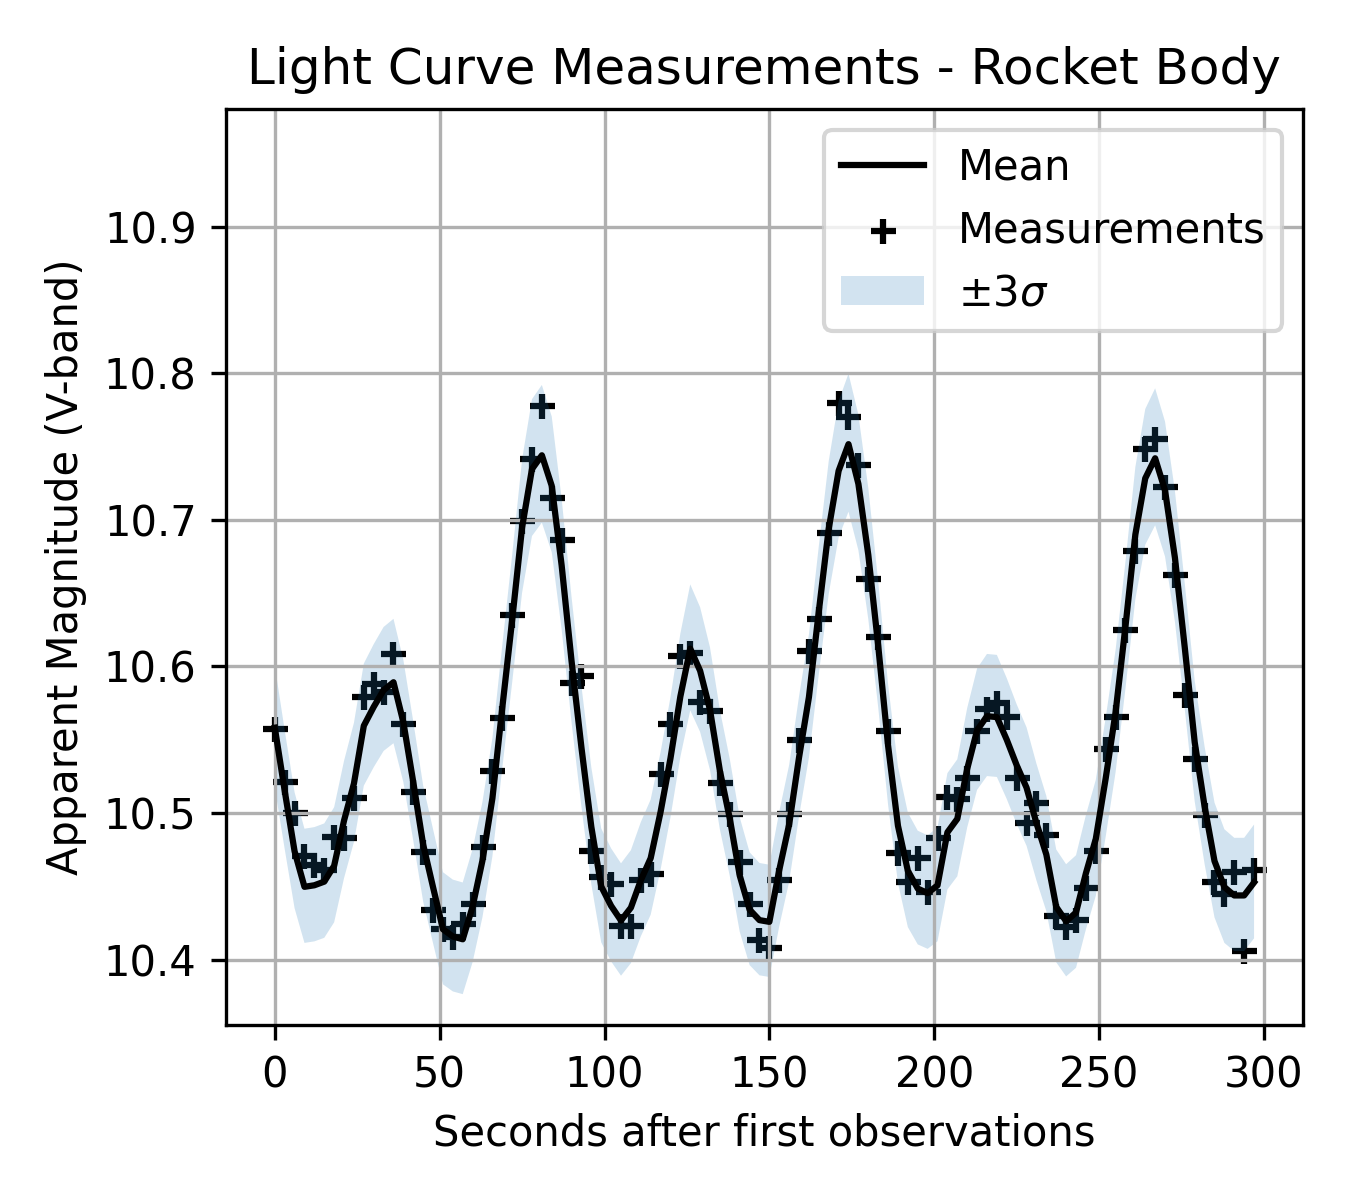
\includegraphics[width=\figmed]{light_curves_mag_rocket_body_sdc.png}
  \caption{Simulated mean and sampled observations for the rocket body in black in V-band magnitude, with the variance included in blue.}
  \label{fig:obs_mag_synth}
\end{figure}

% \begin{figure}[H]
%   \centering
%   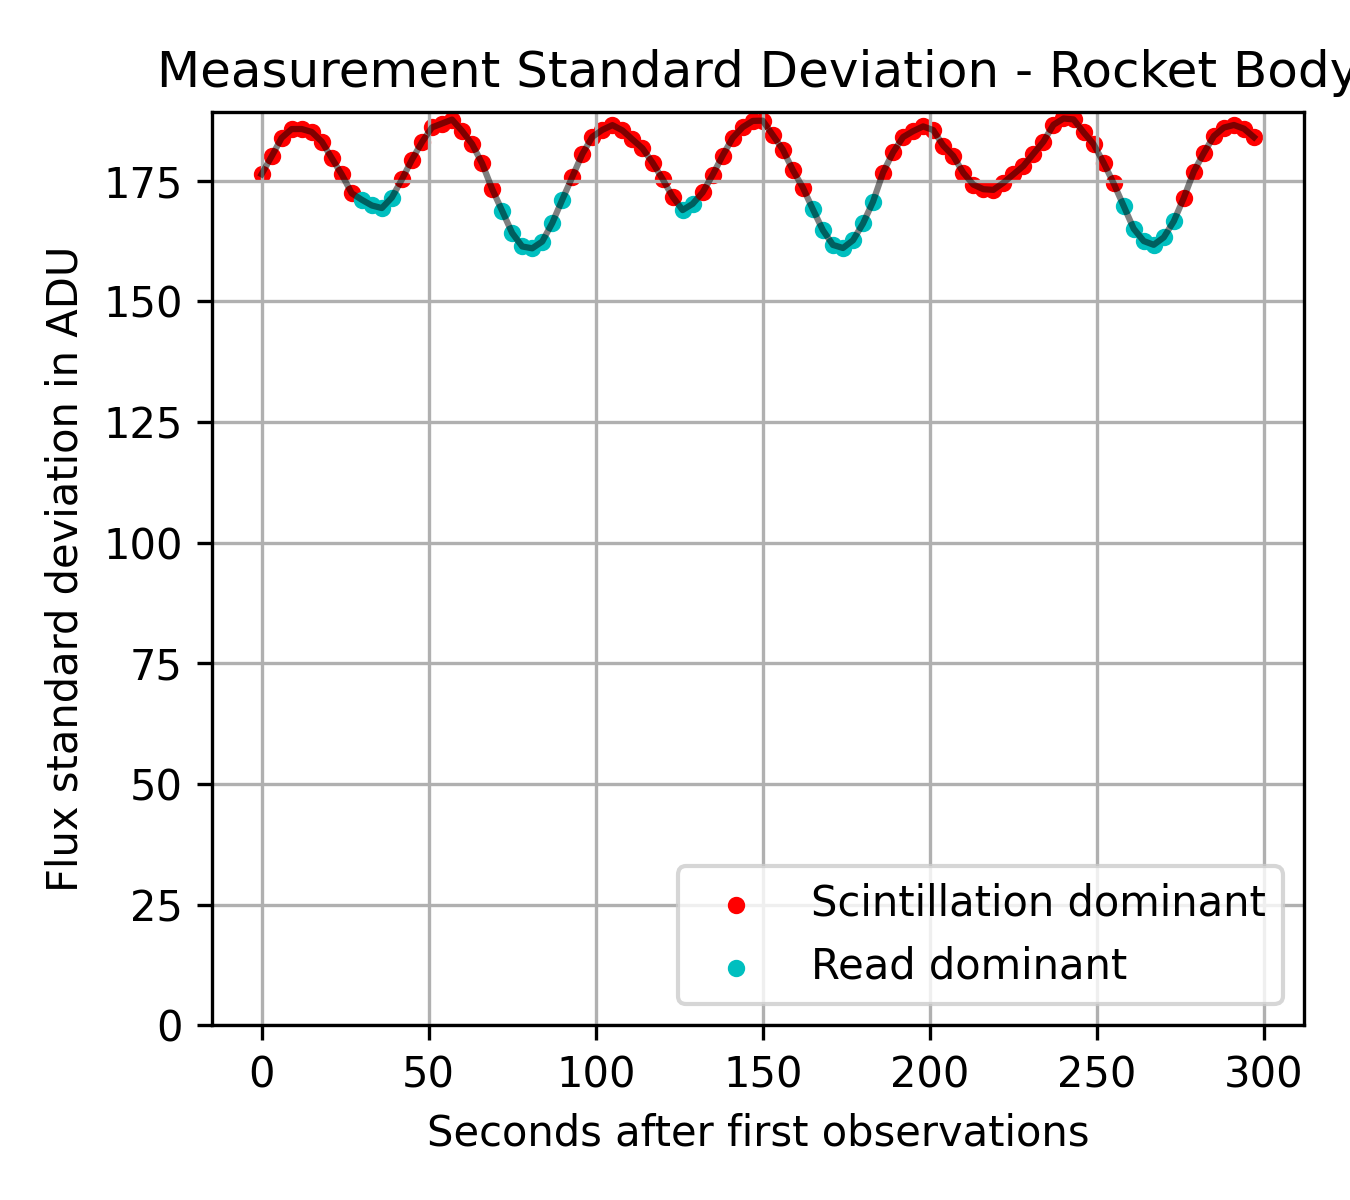
\includegraphics[width=\figsmall]{light_curves_std_rocket_body_sdc.png}
%   \caption{Simulated observed light curve standard deviation computed with Equation \ref{eq:sigma_total}.}
%   \label{fig:obs_std_synth}
% \end{figure}

\subsection{Case 1a and 1b: Synthetic Light Curve Optimization Results}

To emulate the reality that the precise geometry of the observed object is usually uncertain, we use perform attitude inversion with a significantly simplified rocket body model, shown in Figure \ref{fig:rb_models}.

\begin{figure}[H]
  \centering
  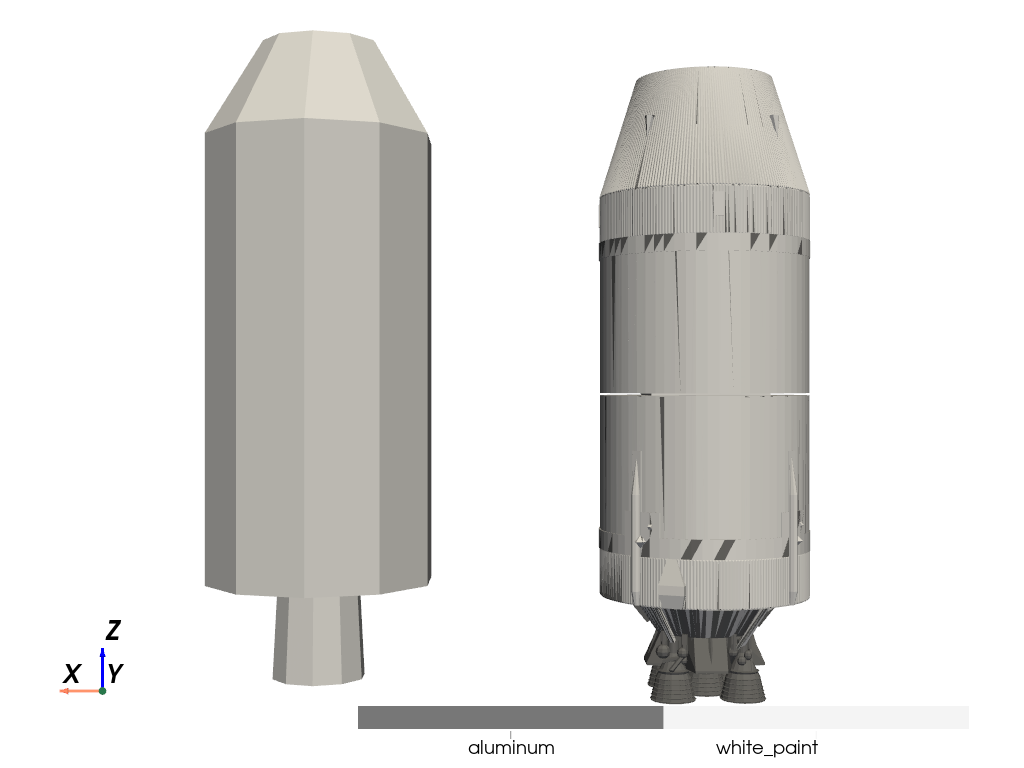
\includegraphics[width=\figmed]{rocket_bodies.png}
  \caption{Simplified rocket body model used for inversion (left) and simulated ground truth model (right).}
  \label{fig:rb_models}
\end{figure}

Two distinct inversion cases are computed. Case 1a presents inversion results given no attitude information besides an estimate of the inertia tensor ratios derived from the known geometry, while Case 1b presents results given good prior attitude state distributions. Tables \ref{tb:case1a_prior} and \ref{tb:case1b_prior} summarize the initial condition sampling strategies employed for each case.

For both cases, a total of $n_\text{sample}=10^5$ initial state samplees are created via the sampling schemes described their respective tables. BFGS minimization is then performed for each initial state sample to locally solve the optimization problem given by Equation \ref{eq:opt_problem}.

\begin{table}[H]
  \centering
  \renewcommand{\arraystretch}{1.3} % Increase row height for better readability
  \caption{Initial condition sampling parameters used for inversion in Case 1a}
  \vspace*{6pt}
  \begin{tabular}{@{} l l @{}}
    \toprule
    Variable & Value \\ \midrule
    $\vctr{p}$ sampling & Uniform, via Equation \ref{eq:mrp_sampler} \\ \grule
    $\vctr{\omega}$ sampling & Uniform, via Equation \ref{eq:omega_sampler} \\ \grule
    $J$ sampling & Gaussian, via Equation \ref{eq:omega_sampler} \\ \grule
    $\sigma_J$ & $0.1$ $[\text{nondim}]$ \\ \grule
    $\norm{\vctr{\omega}}_\text{max}$ & $5.26$ $[\text{deg}\cdot \text{s}^{-1}]$ \\ \brule
  \end{tabular}
  \label{tb:case1a_prior}
\end{table}


\begin{table}[H]
  \centering
  \renewcommand{\arraystretch}{1.3} % Increase row height for better readability
  \caption{Informative prior parameters used for inversion in Case 1b. The standard deviations $\sigma_\omega$ and $\sigma_J$ are for spherically-symmetric Gaussians centered on the ground truth. MRPs are sampled by rotating by $\theta\sim \mathcal{N}(0,\sigma_p)$ degrees away from the ground truth orientation around an axis uniformly sampled on the sphere.}
  \vspace*{6pt}
  \begin{tabular}{@{} l l @{}}
    \toprule
    Variable & Value \\ \midrule
    $\vctr{p}$ sampling & Gaussian, $\sigma_p=20$ $[\text{deg}]$ \\ \grule
    $\vctr{\omega}$ sampling & Gaussian, $\sigma_\omega = 0.1$ $[\text{deg}\cdot\text{s}^{-1}]$ \\ \grule
    $J$ sampling & Gaussian, $\sigma_J = 0.05$ $[\text{nondim}]$ \\ \brule
  \end{tabular}
  \label{tb:case1b_prior}
\end{table}

Solutions are then classified as candidates for the ground truth with $\ell = 1/2$ via Equation \ref{eq:ell_selection_criteria}. Figure \ref{fig:conv_lcs_synth} shows the mean light curves produced by the identified candidate solutions. There is good agreement between the candidate light curves and the observations, indicating that high-quality local minima have been identified.

\begin{figure}[H]
  \centering
  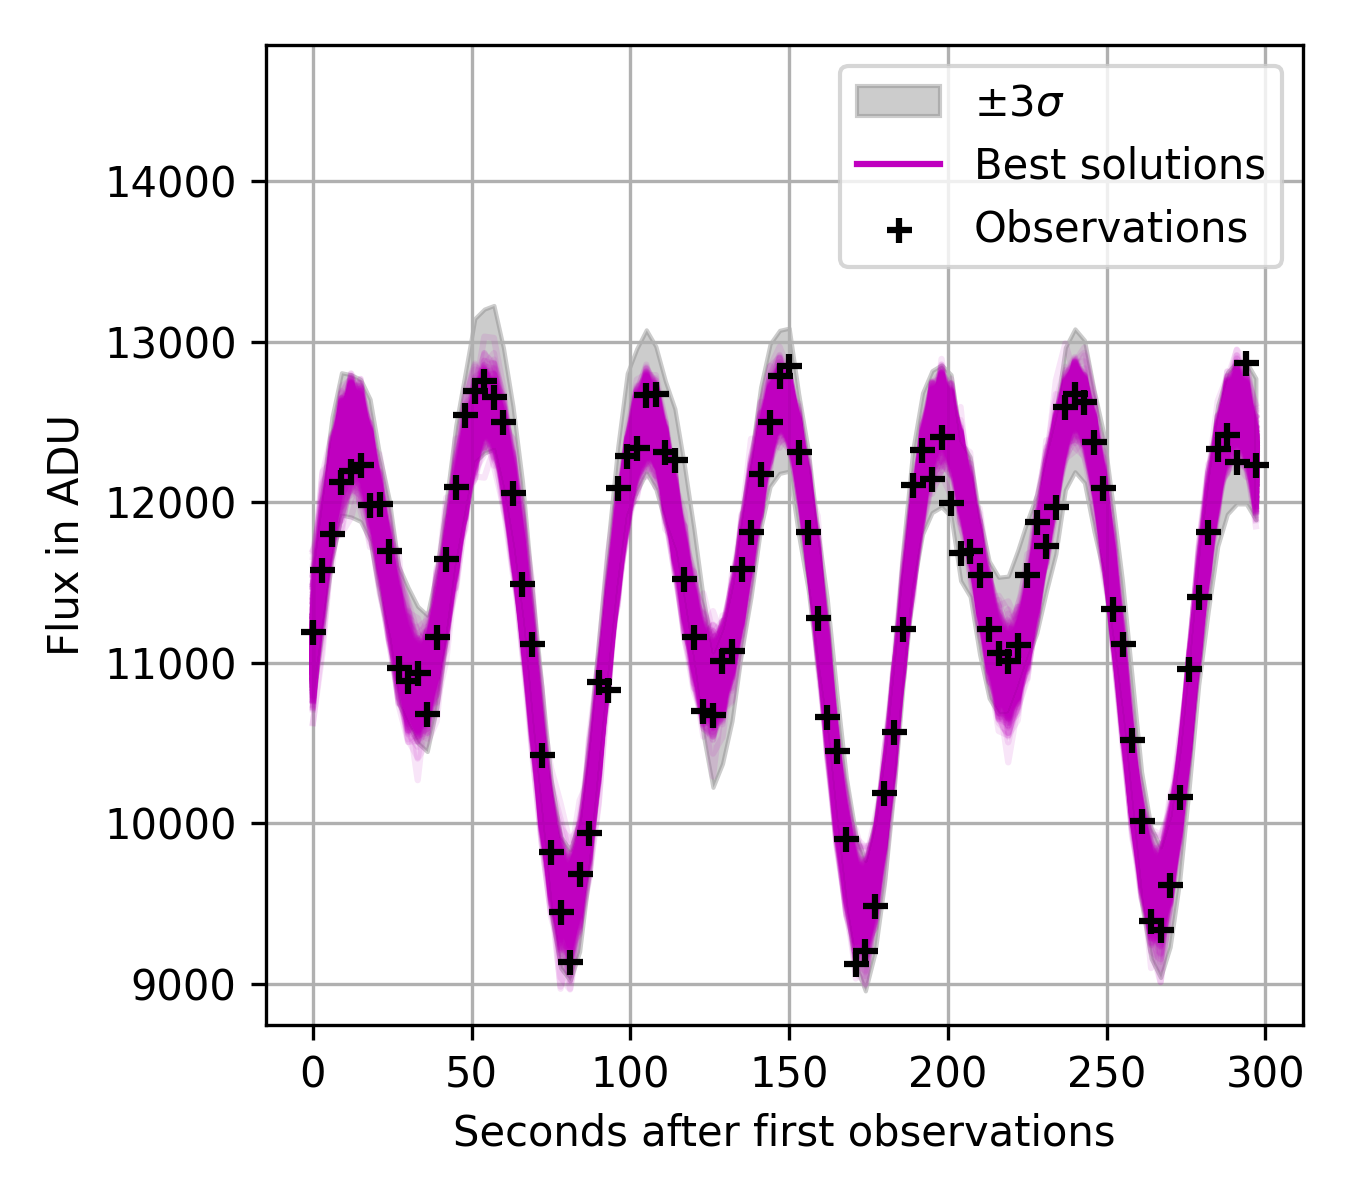
\includegraphics[width=\figbig]{converged_solutions_1_Rocket Body.png}
  \caption{Candidate solution light curves found through BFGS optimization.}
  \label{fig:conv_lcs_synth}
\end{figure}

Figures \ref{fig:sigma_sols1} and \ref{fig:omega_sols1} display the candidate MRP and angular velocity of the candidate solutions determined via the procedure in Section \ref{sec:candidate_sols}. In the left Case 1a figures for orientation and angular velocity, we notice that the ground truth in red lies squarely on a surface containing numerous candidate solutions. This indicates that the local minima have correctly converged to the non-singular subspace of states that approximate the observations well for the assumed shape model. In angular velocity space, shown in Figure \ref{fig:omega_sols1}, most solutions fall onto the surface of two open-ended cylinders -- one with half the radius of the larger cylinder containing the truth. Similarly in orientation space, shown in Figure \ref{fig:sigma_sols1}, the solutions fall on two distinct manifolds, one containing the truth -- likely resulting from a reflection of the object's body frame about the bisector between the Sun and observer vectors \cite{marto2024, burton2024journal}. These additional families of solutions highlight the reality that a wide variety of attitude profiles can produce nearly identical observations.

The Case 1b results on the right within Figures \ref{fig:sigma_sols1} and \ref{fig:omega_sols1} show that the majority of the initial states sampled close to the truth have converged to a local subset of the solution manifolds identified by Case 1a. We should not expect these solutions to have shrunk down exponentially towards the ground truth -- the mismatch in the assumed shape model and the measurement noise inherently limits the minimum size of the feasible solution space.

\begin{figure}[H]
  \centering
  \begin{subfigure}[t]{0.23\textwidth}
    \centering
    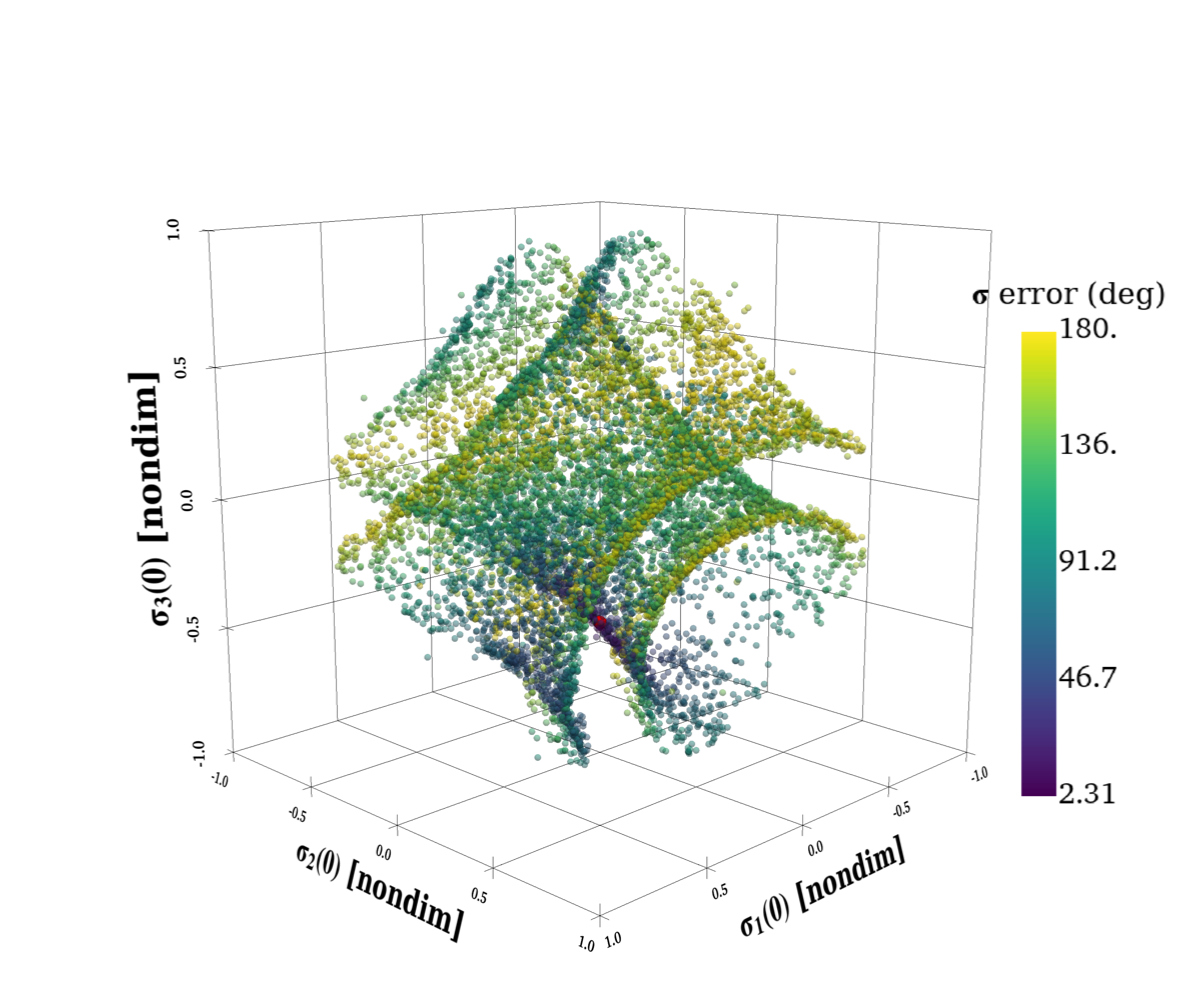
\includegraphics[width=\textwidth]{sigma_solsRocket Body.png}
    \caption{}
    \label{fig:sigma_sols1a}
  \end{subfigure}
  \hfill
  \begin{subfigure}[t]{0.23\textwidth}
    \centering
    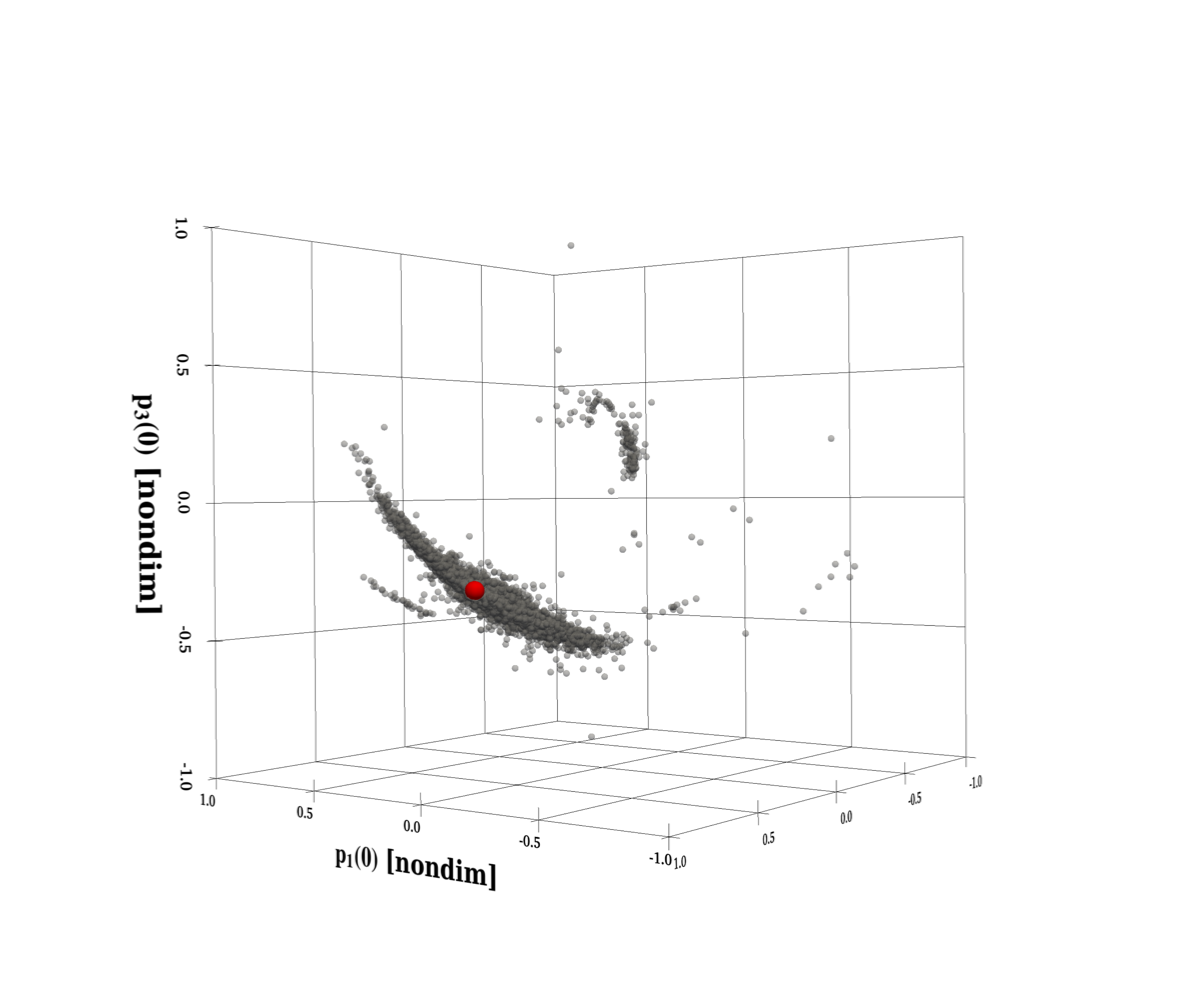
\includegraphics[width=\textwidth]{sigma_solsRocket Body Prior_pin.png}
    \caption{}
    \label{fig:sigma_sols1b}
  \end{subfigure}

  \caption{Candidate solution initial orientation MRP vectors for Cases 1a (left) and 1b (right), with the ground truth highlighted in red.}
  \label{fig:sigma_sols1}
\end{figure}

\begin{figure}[H]
  \centering
  \begin{subfigure}[t]{0.23\textwidth}
    \centering
    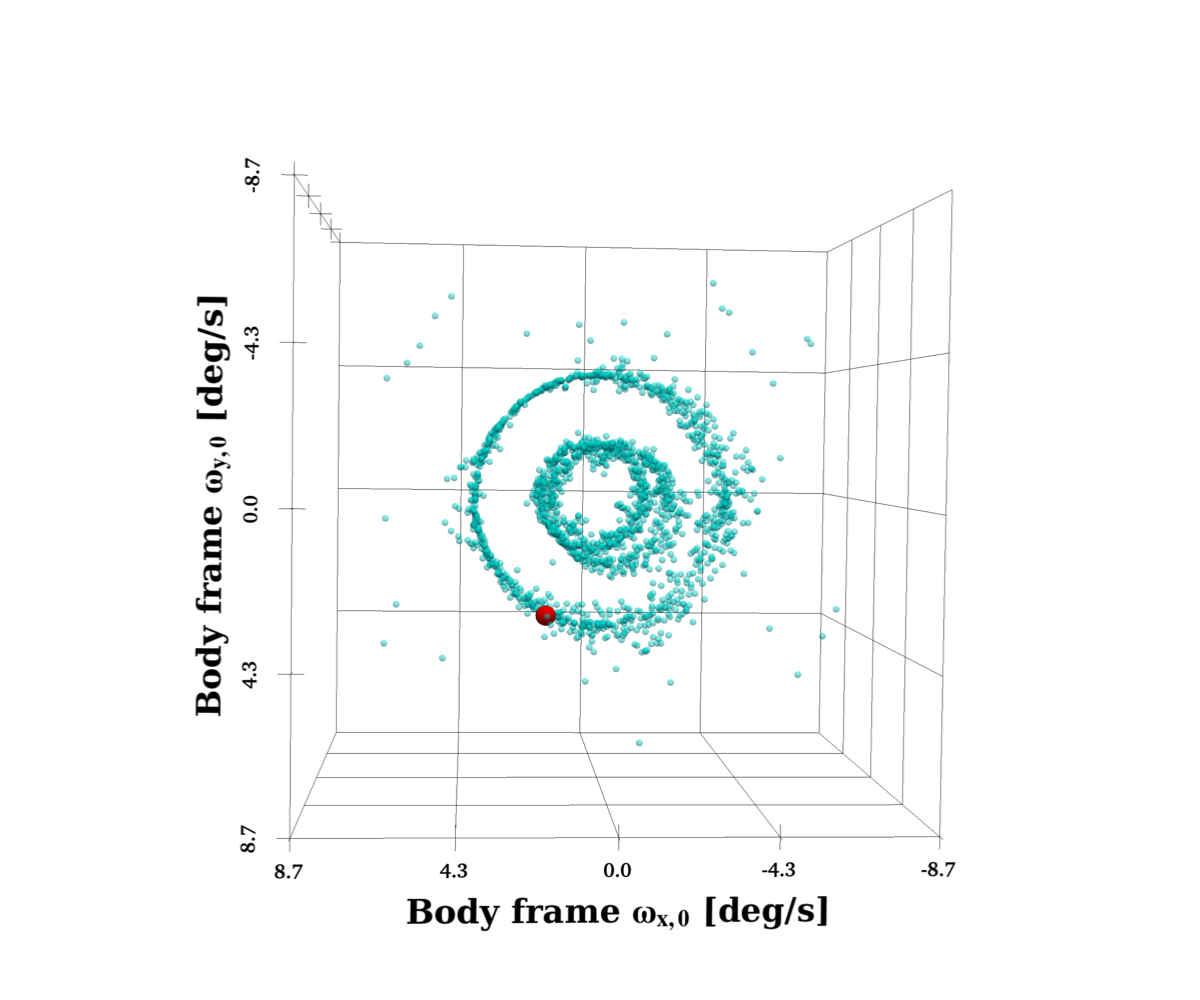
\includegraphics[width=\textwidth]{omega_sols_Rocket Body_pin.png}
    \caption{}
    \label{fig:omega_sols1a}
  \end{subfigure}
  \hfill
  \begin{subfigure}[t]{0.23\textwidth}
    \centering
    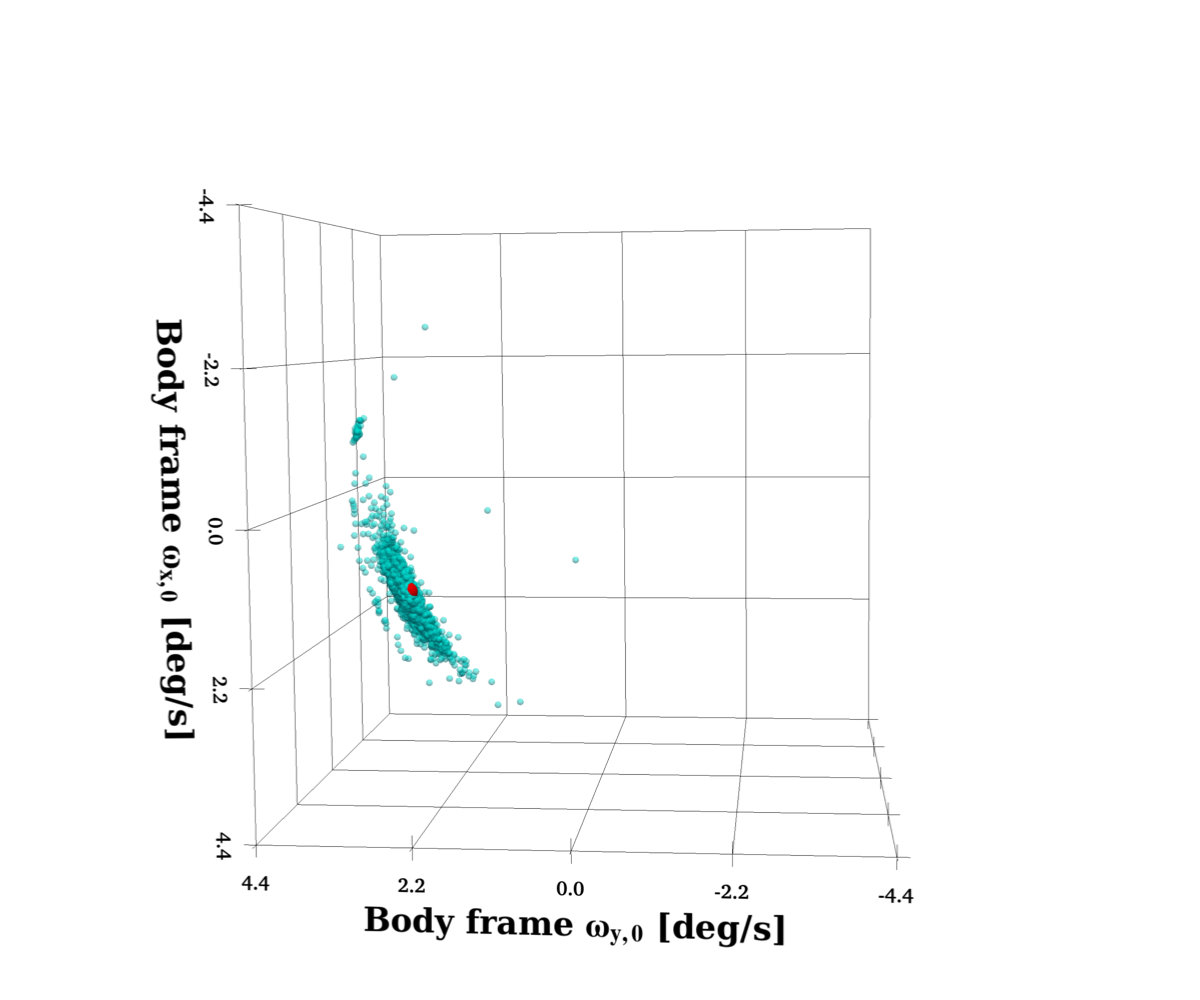
\includegraphics[width=\textwidth]{omega_sols_Rocket Body Prior_pin.png}
    \caption{}
    \label{fig:omega_sols1b}
  \end{subfigure}
  \caption{Candidate solution initial body-frame angular velocity vectors for Cases 1a (left) and 1b (right), with the ground truth highlighted in red. TODO: change the perspective on the angular velocities}
  \label{fig:omega_sols1}
\end{figure}

Figure \ref{fig:i_sols1} displays the inertia tensor solutions for Cases 1a and 1b. Notably, the majority of candidate solutions remain within a few standard deviations of the mean of their initial distribution, with the remaining minority exploring directions that maintain the same precession rate. When a good prior for the other attitude state components is available in Case 1b, the inertia tensor solutions are more well-clustered, although due to the low observability of the rocket body's spin rate in the observed light curve, there are still ambiguous solutions with higher or lower $J_z / J_x$ values.

\begin{figure}[H]
  \centering
  \begin{subfigure}[t]{0.23\textwidth}
    \centering
    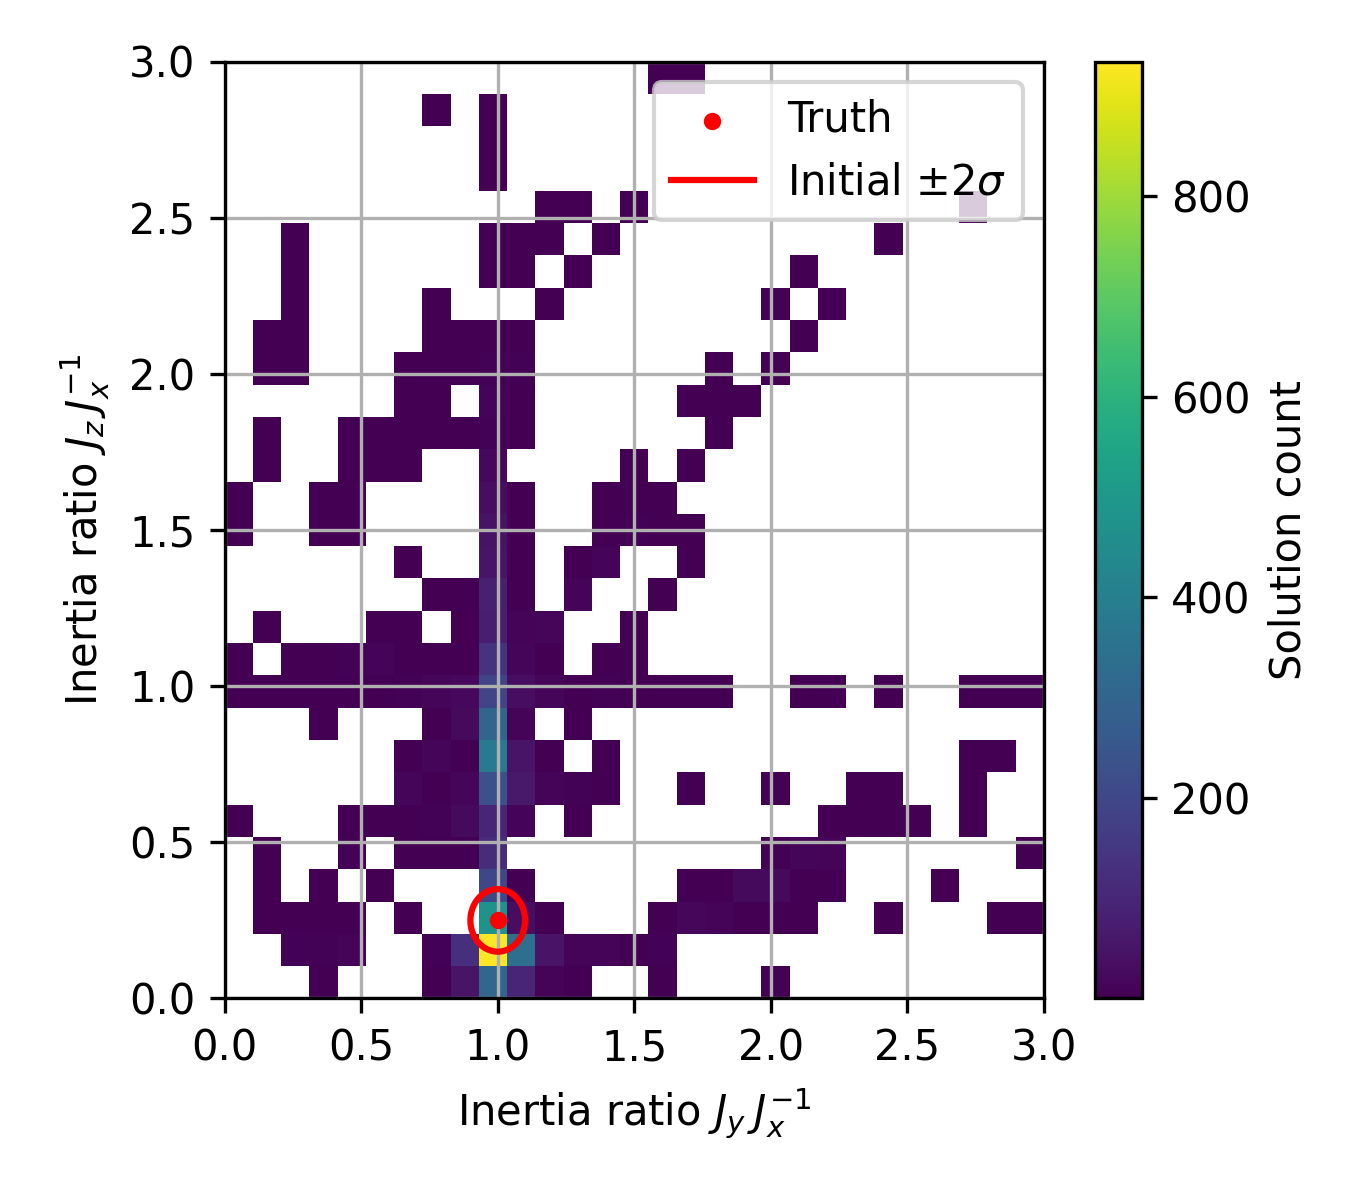
\includegraphics[width=\textwidth]{converged_solutions_2_Rocket Body.png}
    \caption{}
    \label{fig:i_sols1a}
  \end{subfigure}
  \hfill
  \begin{subfigure}[t]{0.23\textwidth}
    \centering
    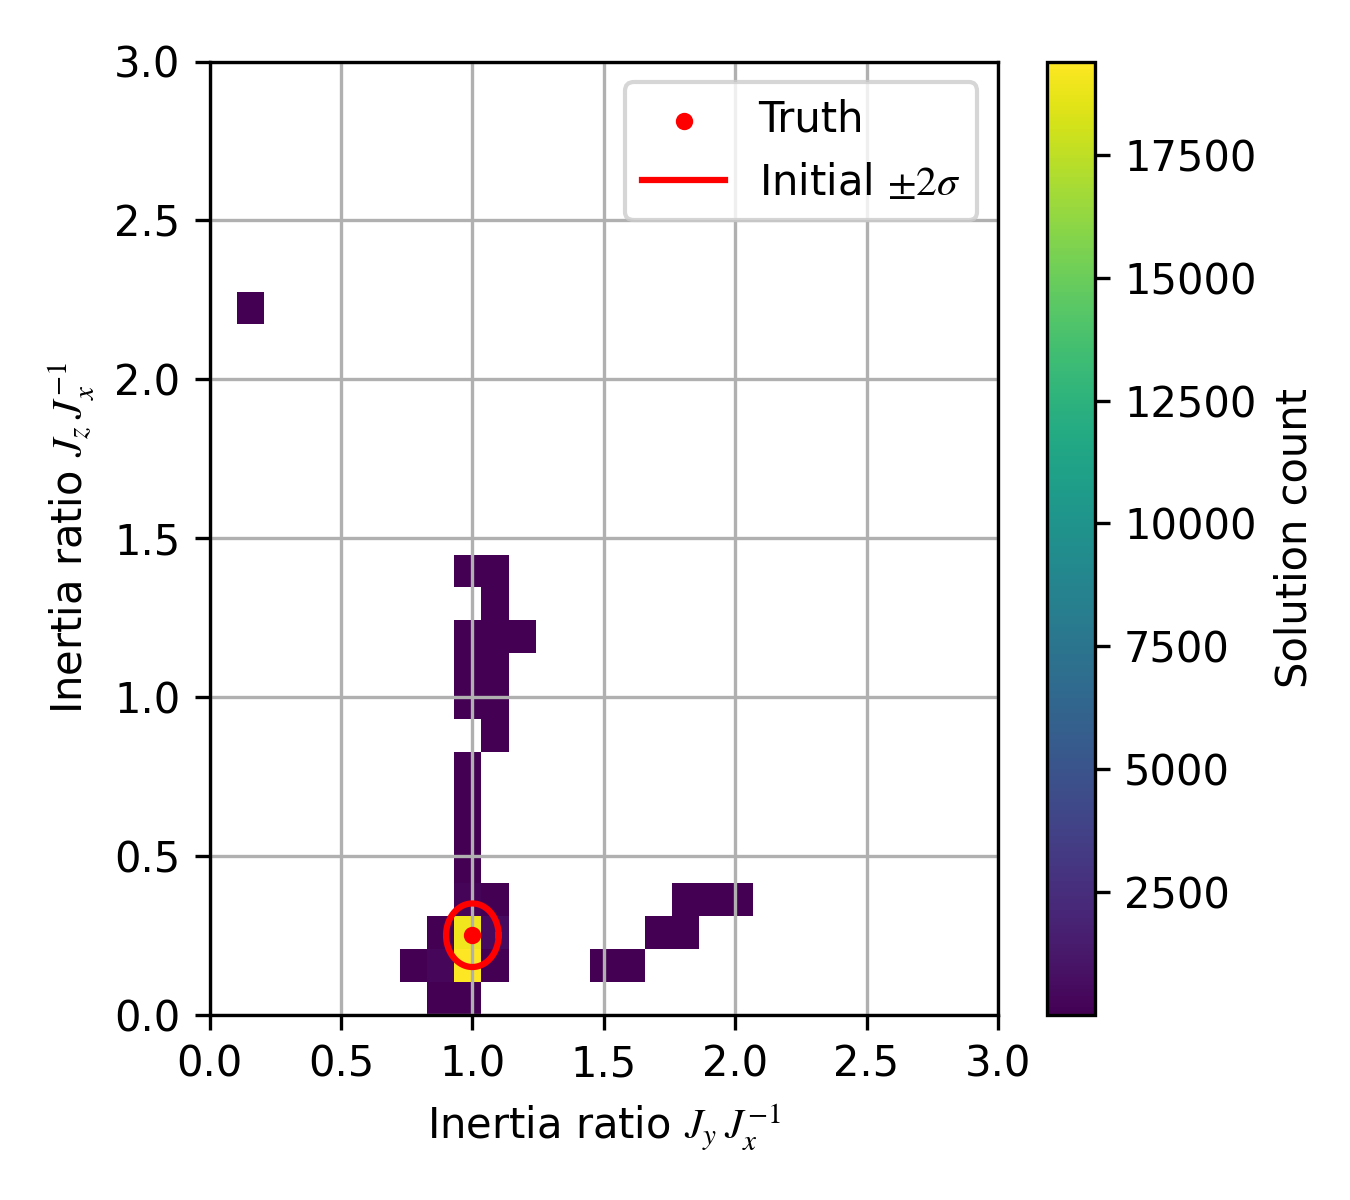
\includegraphics[width=\textwidth]{converged_solutions_2_Rocket Body Prior.png}
    \caption{}
    \label{fig:i_sols1b}
  \end{subfigure}
  \caption{Candidate solution inertia ratios for Cases 1a (left) and 1b (right), with the ground truth highlighted in red.}
  \label{fig:i_sols1}
\end{figure}

Figure \ref{fig:w_vs_ang_error_sols1} summarizes the distribution of candidate solutions with respect to the ground truth by displaying the angular velocity magnitude error and angular orientation error compared to the ground truth. Case 1a shows significant variability in angular velocity magnitude, although this is almost entirely due to the unobservability of the spin rate about the object's axis of symmetry in the light curve. The mean precession rate error is low at $0.3\%$. Due to the underdetermined orientation solution space, there are far more solutions at high angular offsets from the truth orientation, leading to a large mean angular error of $126^\circ$. For Case 1b, the mean orientation error is much lower at $18^\circ$, although convergence here is still inherently limited by the noisy measurements and model mismatch.

\begin{figure}[H]
  \centering
  \begin{subfigure}[t]{0.23\textwidth}
    \centering
    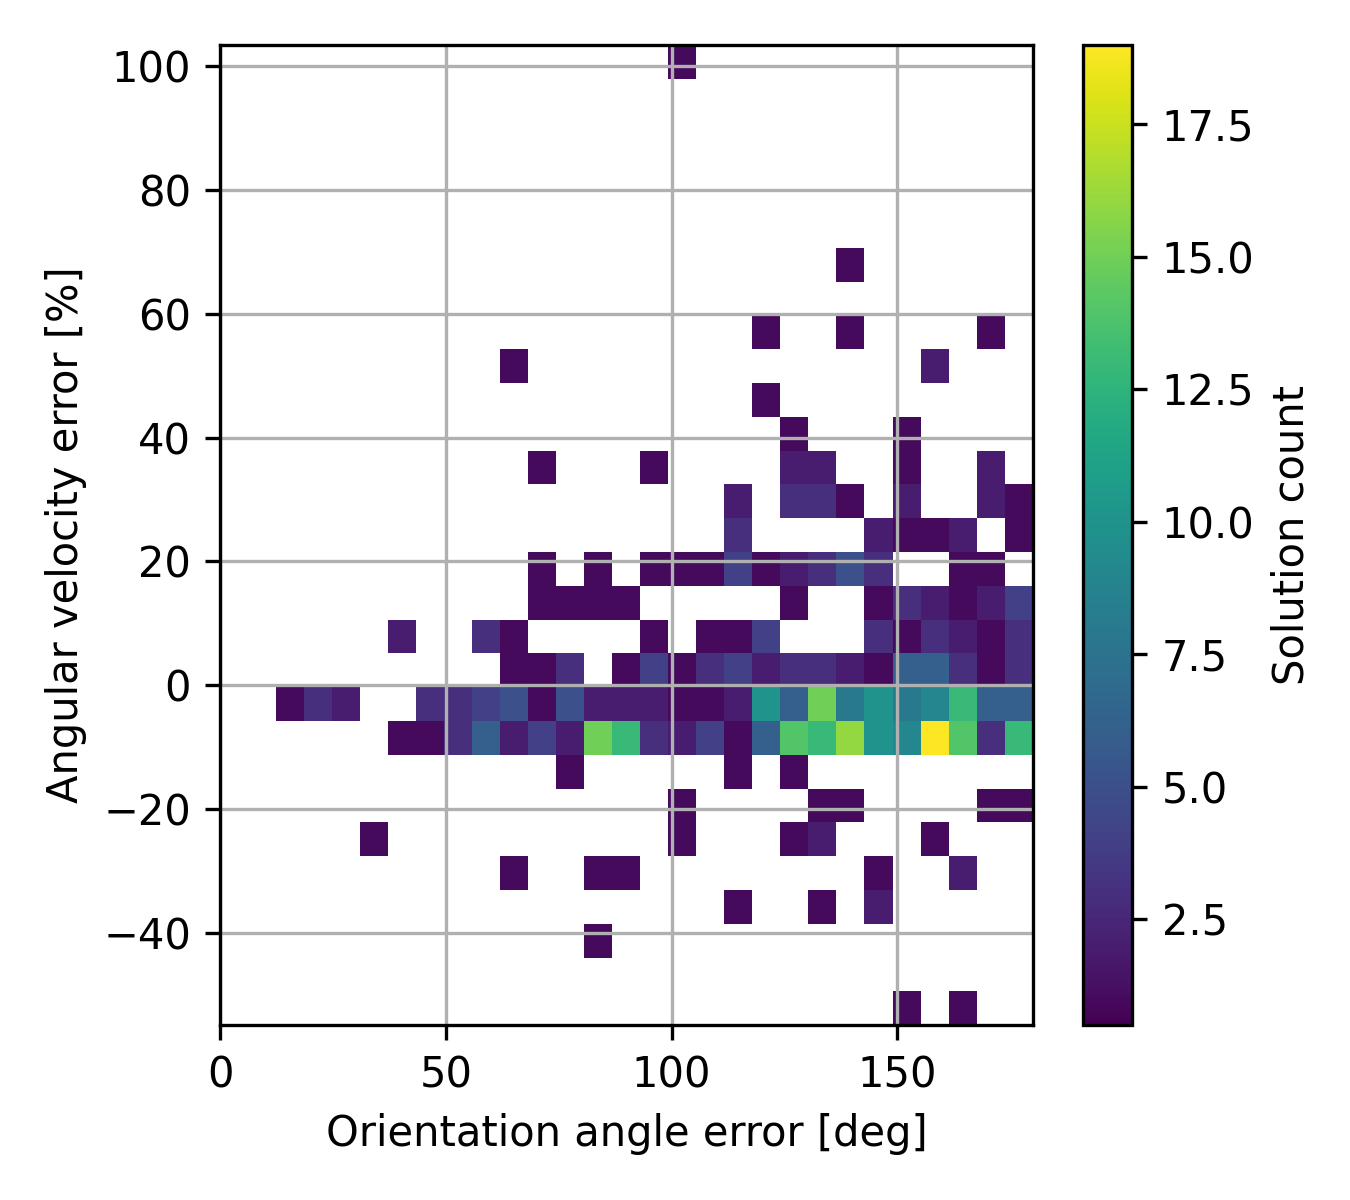
\includegraphics[width=\textwidth]{converged_solutions_3_Rocket Body.png}
    \caption{}
    \label{fig:w_vs_ang_error_sols1a}
  \end{subfigure}
  \hfill
  \begin{subfigure}[t]{0.23\textwidth}
    \centering
    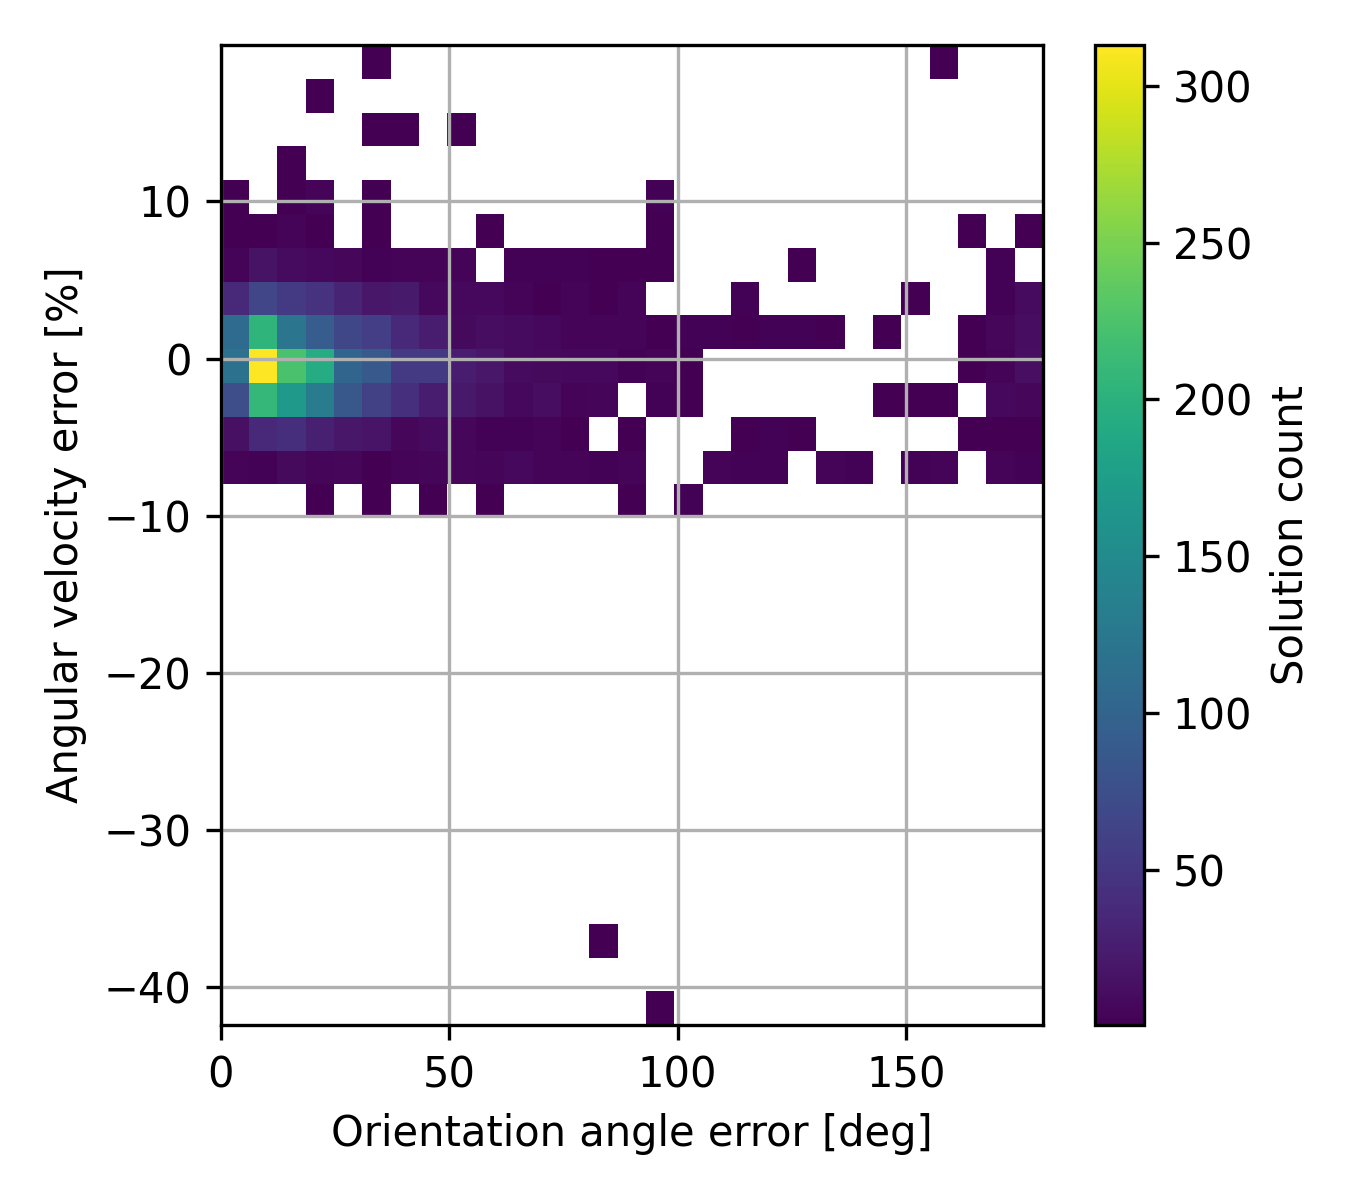
\includegraphics[width=\textwidth]{converged_solutions_3_Rocket Body Prior.png}
    \caption{}
    \label{fig:w_vs_ang_error_sols1b}
  \end{subfigure}

  \caption{Candidate solution angular orientation error and angular velocity magnitudes for Cases 1a (left) and 1b (right) compared to the ground truth}
  \label{fig:w_vs_ang_error_sols1}
\end{figure}

% While the state vectors of the candidate solutions do not uniquely indicate the ground truth, the object's precession rate is estimated

% \begin{figure}[H]
%   \centering
%   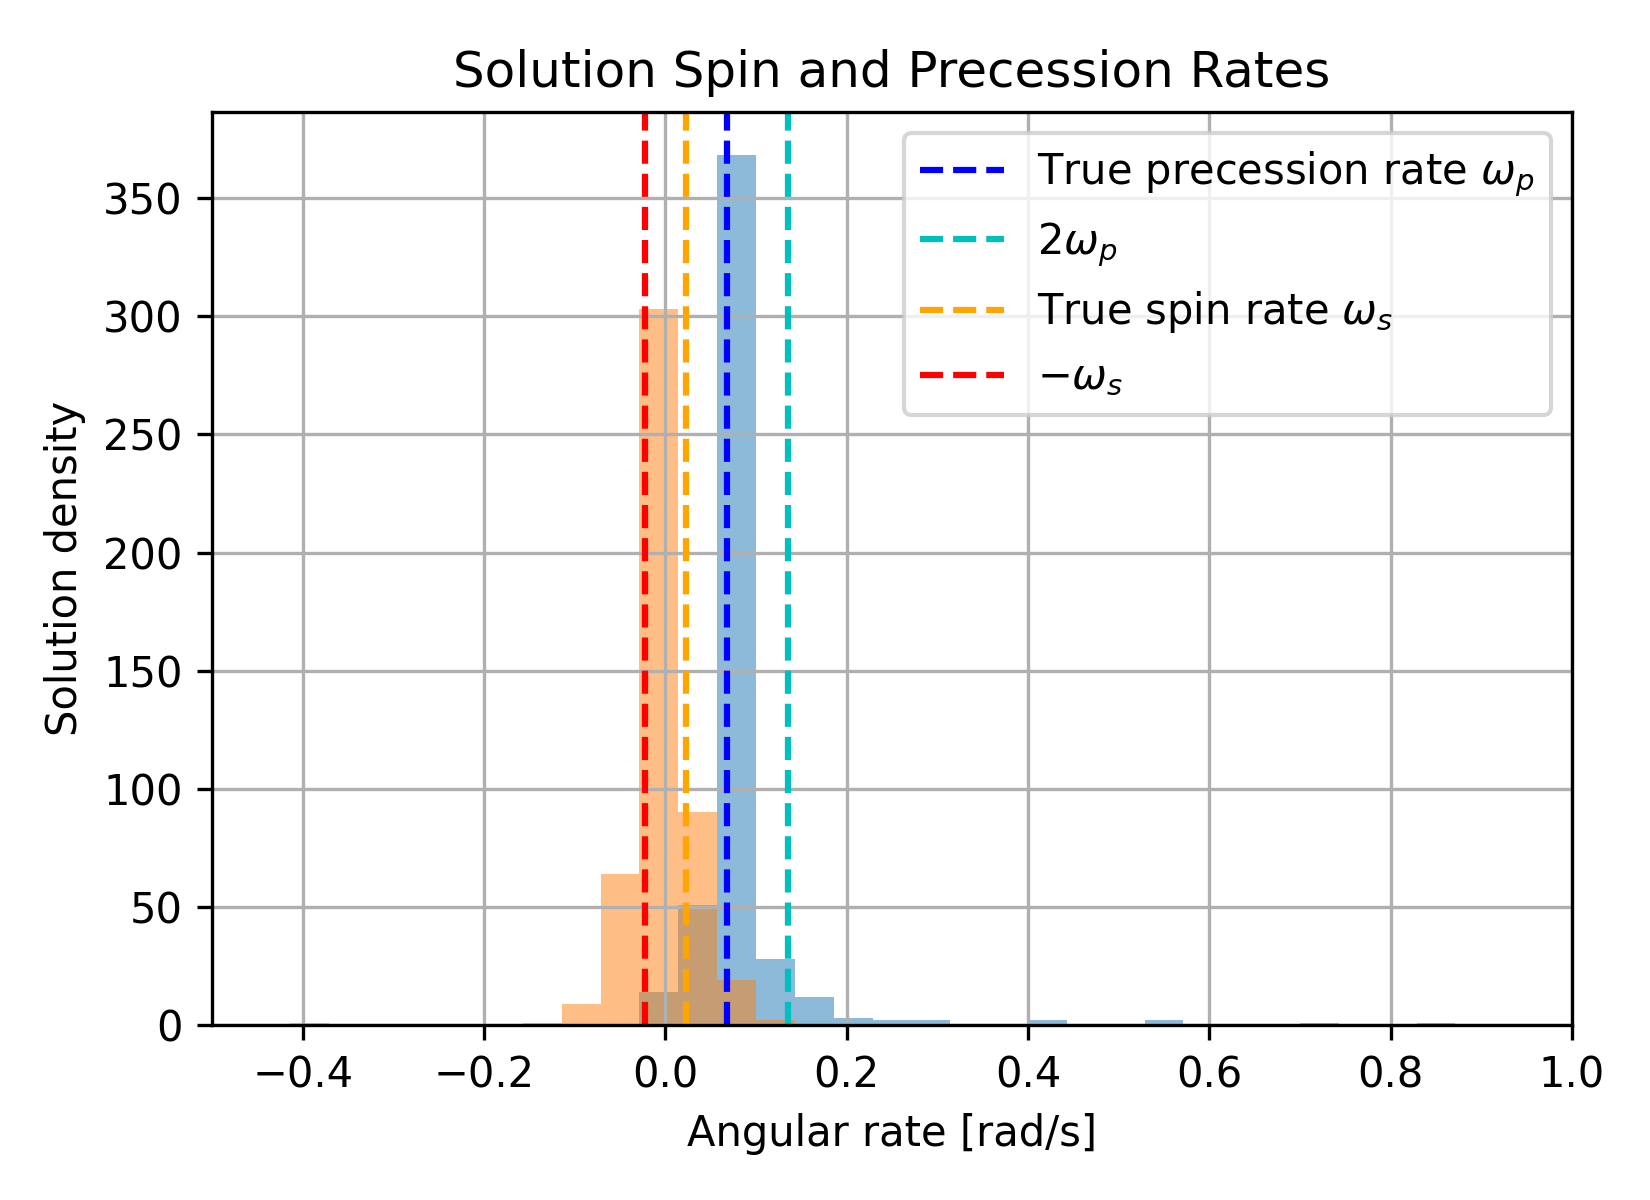
\includegraphics[width=\figsmall]{spin_proc_Rocket Body.png}
%   \caption{Converged solution body frame spin and precession rates.}
%   \label{fig:spin_proc1}
% \end{figure}

\section{Attitude Inversion Results for Real Data} \label{sec:real_results}

% The two objects selected for study in this work are a Delta I upper stage and the ECHOSTAR 2 satellite.

\subsection{Case 2: Delta I Upper Stage}

In Case 2, we perform attitude inversion on real data observed for a Delta I upper stage rocket body. The chosen Delta I upper stage (COSPAR ID 1984-115C) is a Star-37E \cite{delta3914_astronautix} solid fuel apogee kick motor, displayed in Figure \ref{fig:star37e}. It is $d=0.93$ meters in diameter and is approximately $h=1.7$ meters in length \cite{star37e_astronautix, star37_gunter}.

\begin{figure}[H]
  \centering
  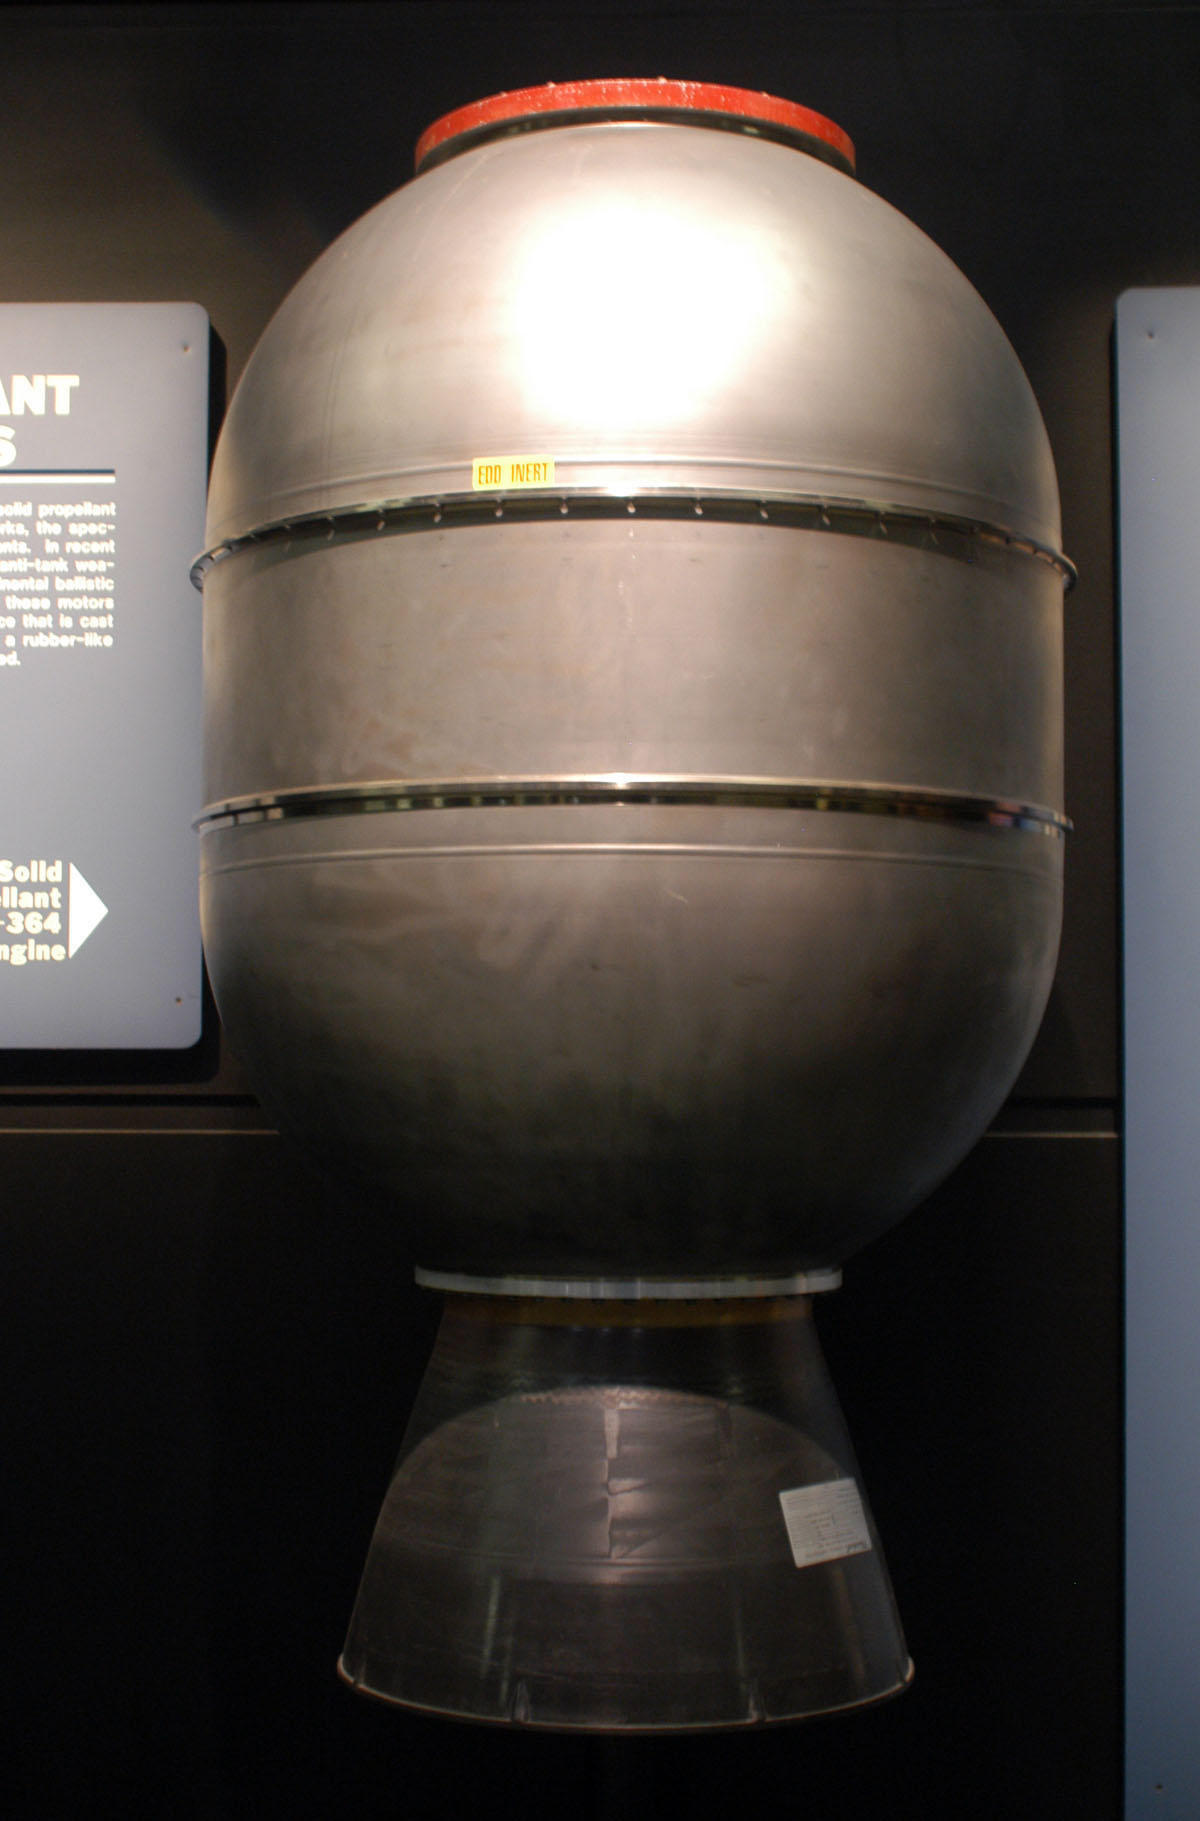
\includegraphics[width=0.25\textwidth]{star37e.JPG}
  \caption{Star-37E upper stage \cite{star37_af}.}
  \label{fig:star37e}
\end{figure}

\begin{figure}[H]
  \centering
  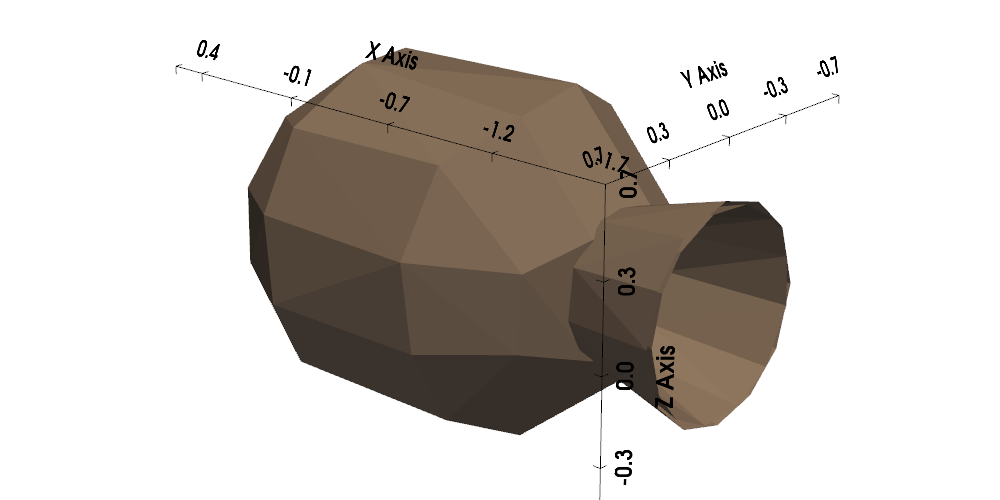
\includegraphics[width=\figbig]{sphx_glr_plot_models_002.png}
  \caption{Simplified Star-37E model used for inversion.}
  \label{fig:star37e_simple}
\end{figure}

We compute the inertia tensor of the Star-37E by approximating its geometry as a hollow cylinder of the same aspect ratio such that \cite{serway2019}:

\begin{align}
 J_a &= \frac{1}{2} m \left(r_o^2+r_i^2\right) \\
 J_t &= \frac{1}{12} m \left(3 \left(r_o^2+r_i^2\right) + h^2\right) \\
 J_\text{R/B} &= \text{diag} \left(J_a, J_t, J_t\right).
\end{align}

Here, we choose the inner radius to be $r_i=0.45d$, the outer radius to be $r_o=0.5d$, and $m=1$ kilogram -- dividing each moment of inertia by a constant does not change the dynamics -- yielding $J_a = 15.3 \: [kg \cdot m^2]$ and $J_t = 27.9 \: [kg \cdot m^2]$. Table \ref{tb:case2_in} summarizes the light curve observations that result in the extracted measurements displayed in Figure \ref{fig:rb_lc_obs}.

\begin{table}[H]
  \centering
  \renewcommand{\arraystretch}{1.3} % Increase row height for better readability
  \caption{Delta I rocket body observation characteristics}
  \vspace*{6pt}
  \begin{tabular}{@{} l l @{}}
    \toprule
    Variable & Value \\ \midrule
    Target COSPAR ID & 1984-115C \\ \grule
    First obs.\ (UTC) & Mar 2, 2025 01:53:30.251 \\ \grule
    Light curve duration & $7.5$ minutes \\ \grule
    Observations & $100$ ($92$ extracted) \\ \grule
    Obs.\ frequency & $0.222$ Hz \\ \grule
    Integration time & $3$ seconds \\ \brule
  \end{tabular}
  \label{tb:case2_in}
\end{table}

\begin{figure}[H]
  \centering
  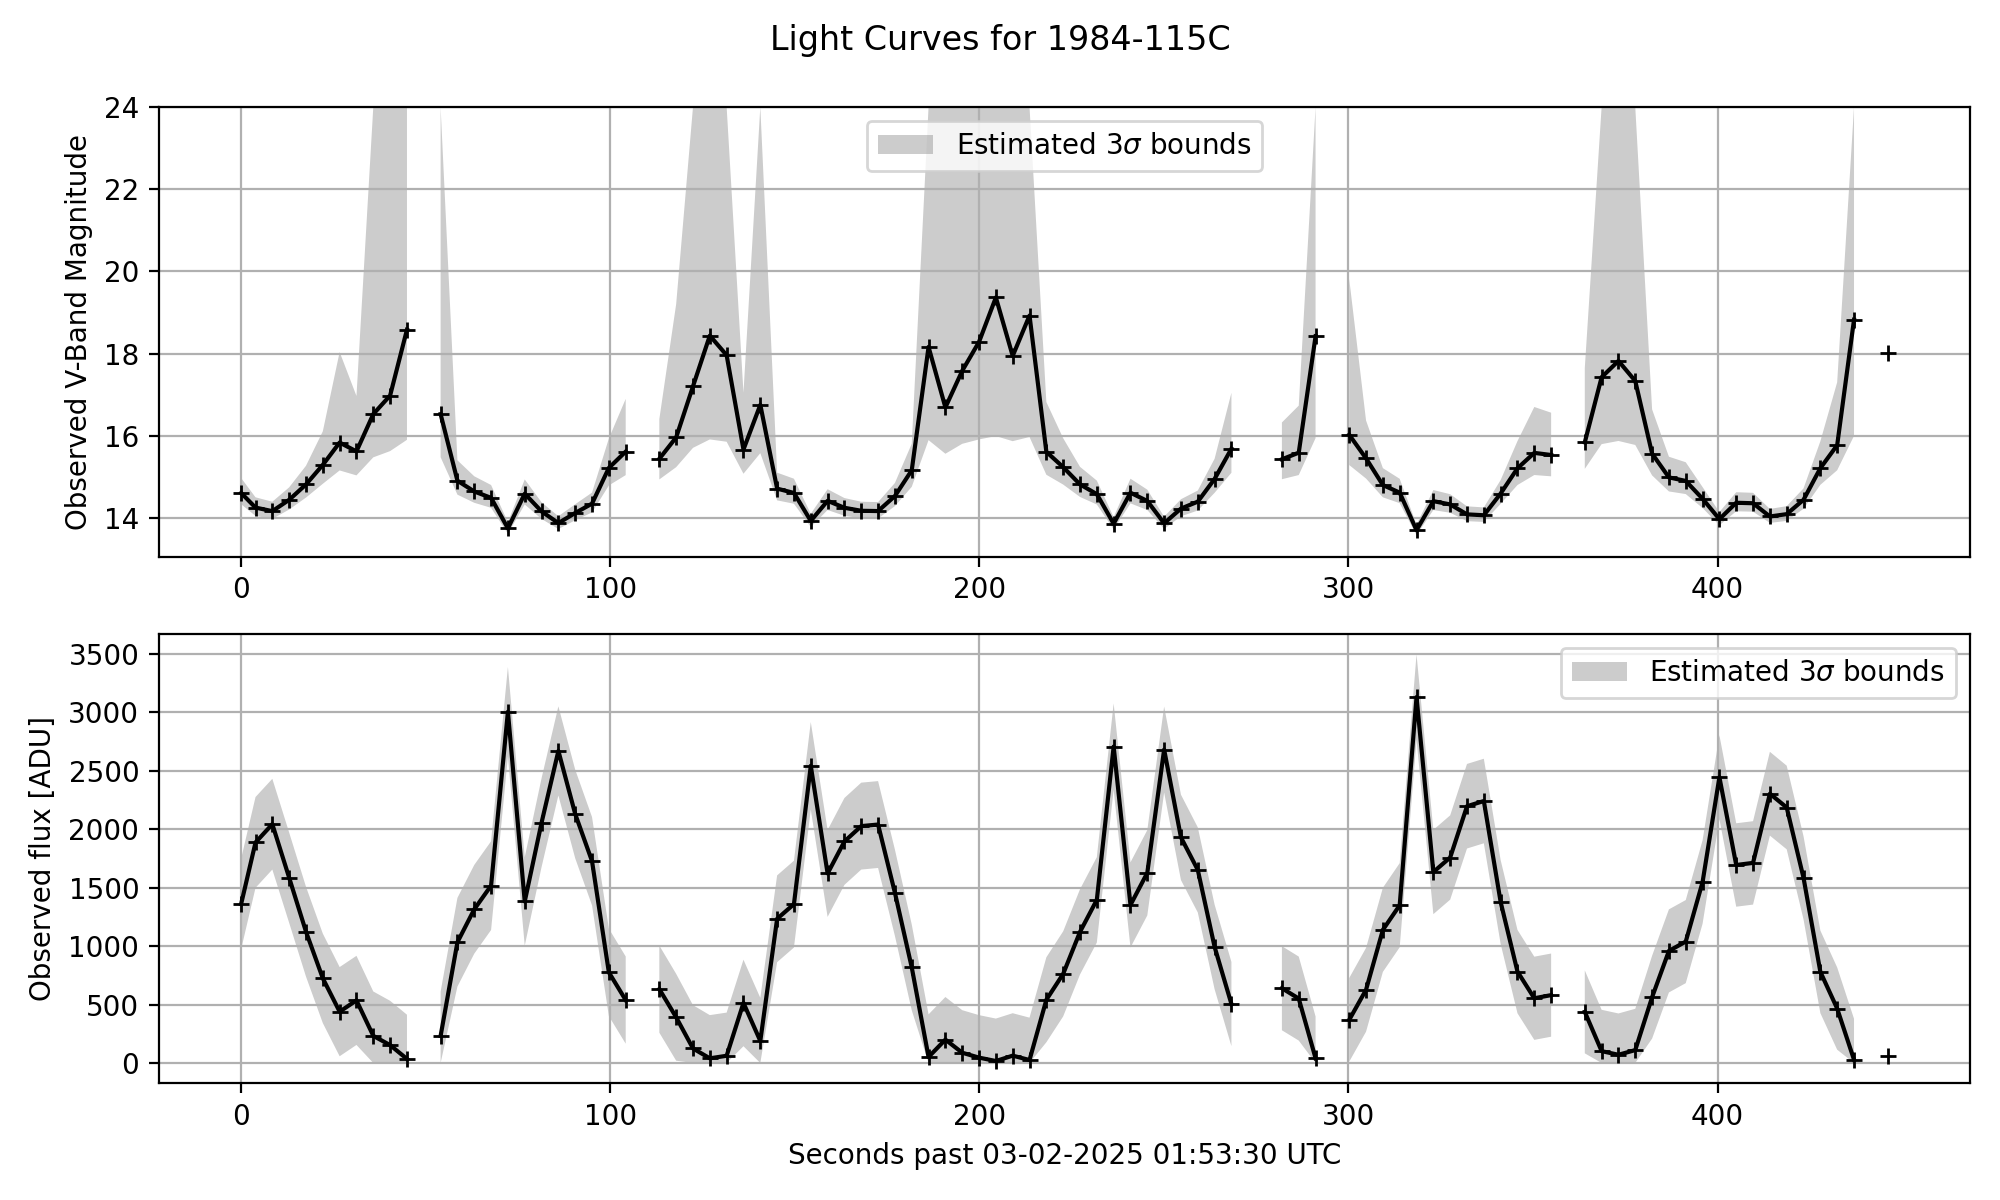
\includegraphics[width=\figbig]{sphx_glr_plot_lcs_001_2_00x.png}
  \caption{Selected light curve for the Delta I (Star-37E) rocket body, observed by the Purdue Optical Ground Station}
  \label{fig:rb_lc_obs}
\end{figure}

This light curve shows clear periodicity, but has a high measurement standard deviation and a relatively low sampling rate due to the object's low brightness and the sensor readout time. Inversion is performed using $n_\text{sample}=10^4$ samples with the material and angular velocity assumptions listed in Table \ref{tb:case2_ass}. As in Case 1a, orientation and angular velocity states are sampled via Equations \ref{eq:mrp_sampler} and \ref{eq:omega_sampler}, respectively. All initial inertia tensor samples are set to the estimated $J_\text{R/B}$. The candidate solution results are presented in terms of their mean light curves in Figure \ref{fig:case2_s}, orientation MRPs and angular velocities in Figure \ref{fig:case2_pw}, and inertia ratios in Figure \ref{fig:case2_i}.

\begin{table}[H]
  \centering
  \renewcommand{\arraystretch}{1.3} % Increase row height for better readability
  \caption{Delta I rocket body inversion assumptions}
  \vspace*{6pt}
  \begin{tabular}{@{} l l @{}}
    \toprule
    Variable & Value \\ \midrule
    Uniform BRDF & $C_d=0.2$, $C_s=0.8$, $n=30$ \\ \grule
    $\norm{\vctr{\omega}}_\text{max}$ & $6.93$ $\text{deg} \cdot \text{s}^{-1}$ \\ \grule
    $\ell$ & $1/100$ \\ \brule
  \end{tabular}
  \label{tb:case2_ass}
\end{table}

\begin{figure}[H]
  \centering
  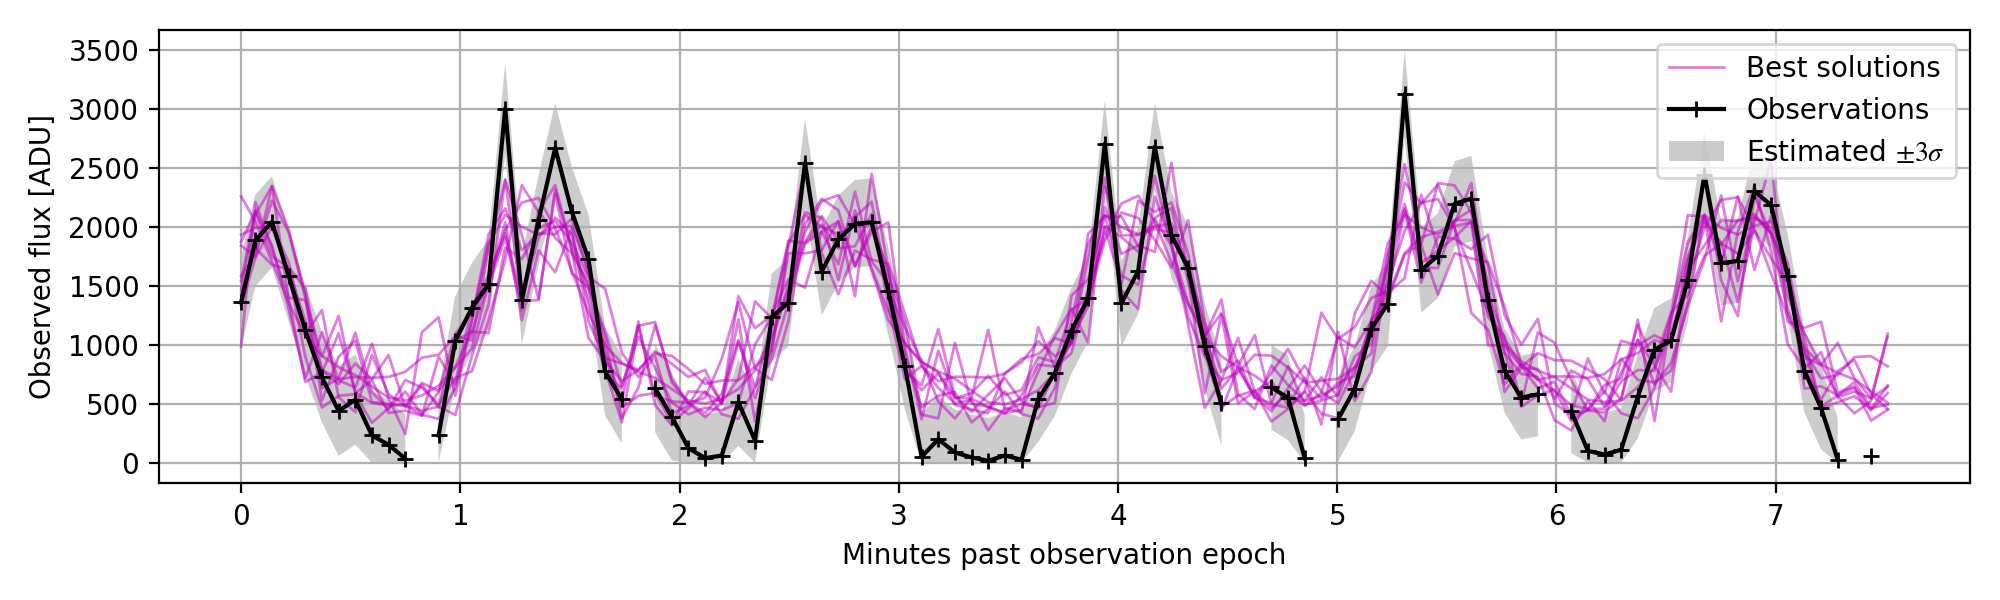
\includegraphics[width=\figbig]{sphx_glr_results_002_2_00x.png}
  \caption{Candidate solution light curves compared to the real measurements in ADU for the Delta I (Star-37E) rocket body.}
  \label{fig:case2_s}
\end{figure}

% \begin{figure}[H]
%   \centering
%   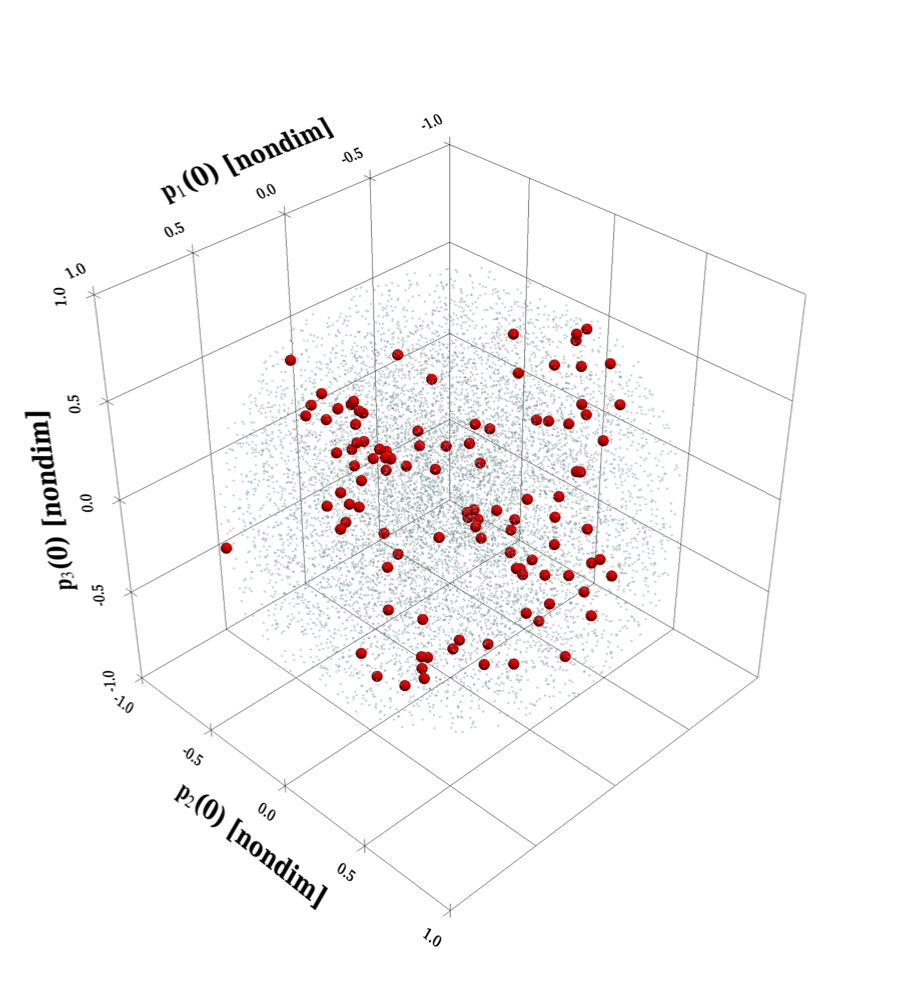
\includegraphics[width=\figmed]{sphx_glr_results_006.png}
%   \caption{}
%   \label{fig:case2_p}
% \end{figure}

\begin{figure}[H]
  \centering
  \begin{subfigure}[t]{0.23\textwidth}
    \centering
    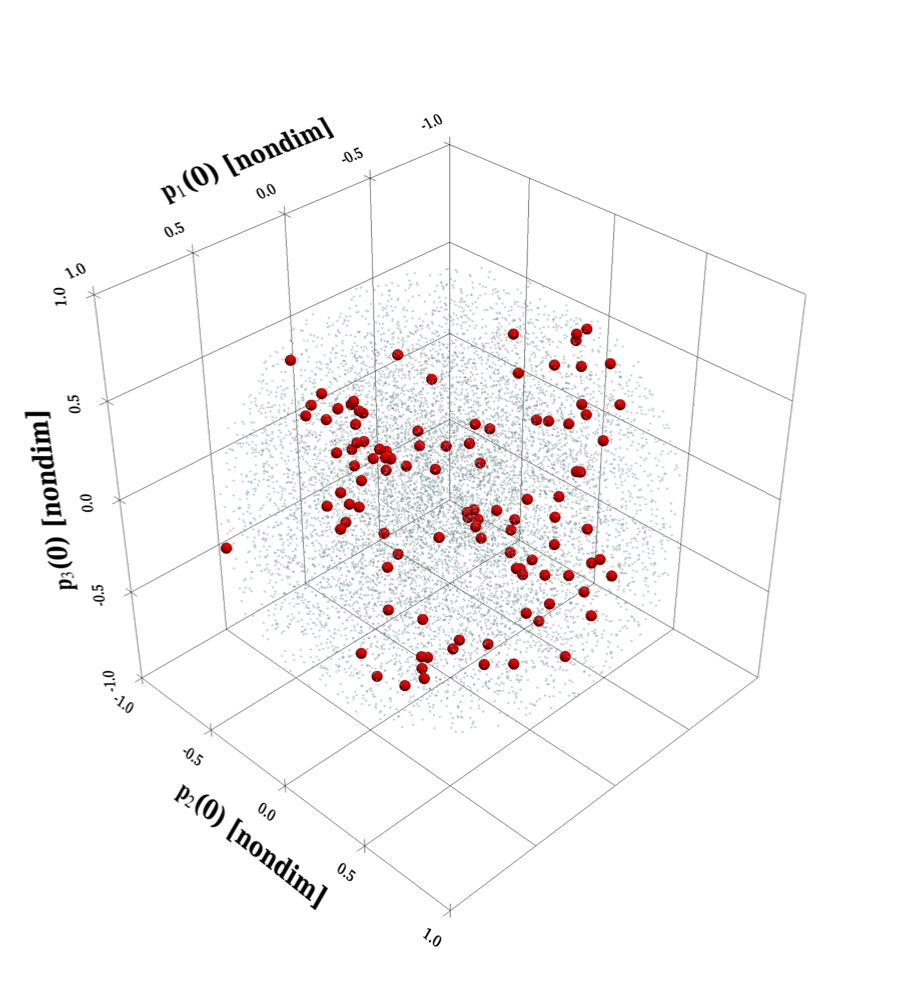
\includegraphics[width=\textwidth]{sphx_glr_results_006.png}
    \caption{}
    \label{fig:case2_pwa}
  \end{subfigure}
  \hfill
  \begin{subfigure}[t]{0.23\textwidth}
    \centering
    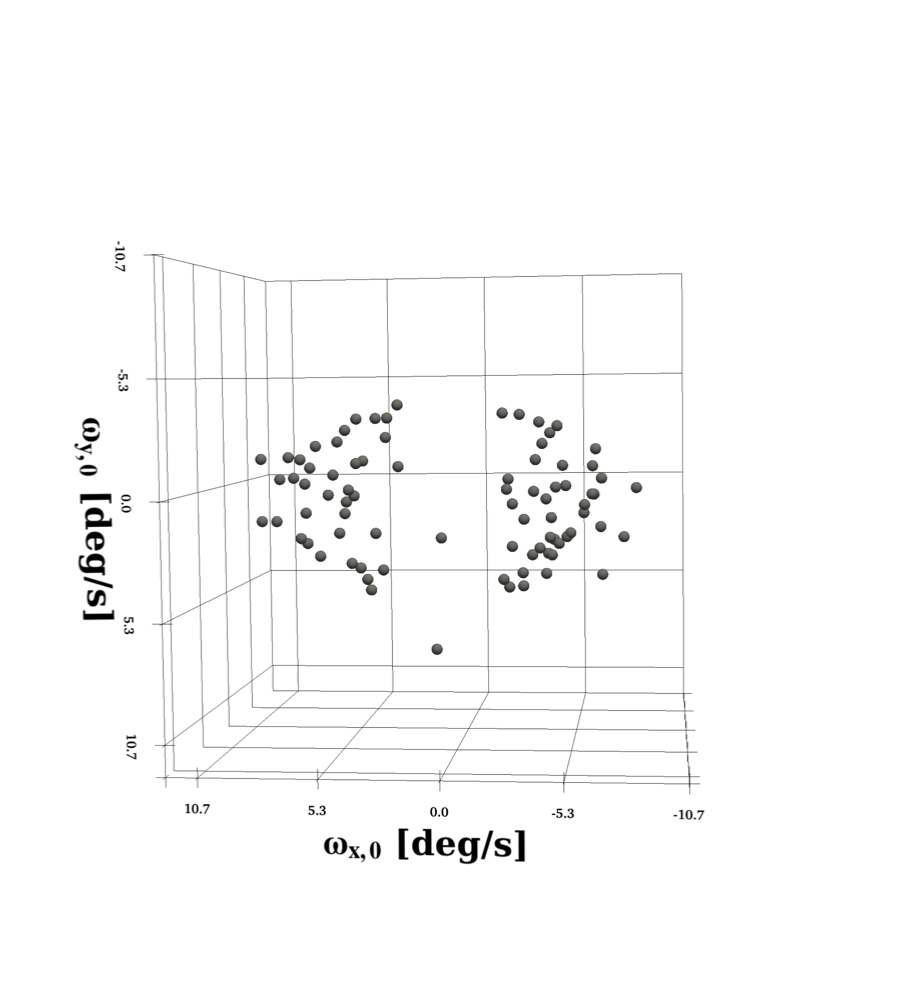
\includegraphics[width=\textwidth]{delta_ang_vel_pin.png}
    \caption{}
    \label{fig:case2_pwb}
  \end{subfigure}

  \caption{Candidate solution orientation MRPs (left) and angular velocity vectors (right) for the Delta I (Star-37E) rocket body}
  \label{fig:case2_pw}
\end{figure}

% \begin{figure}[H]
%   \centering
%   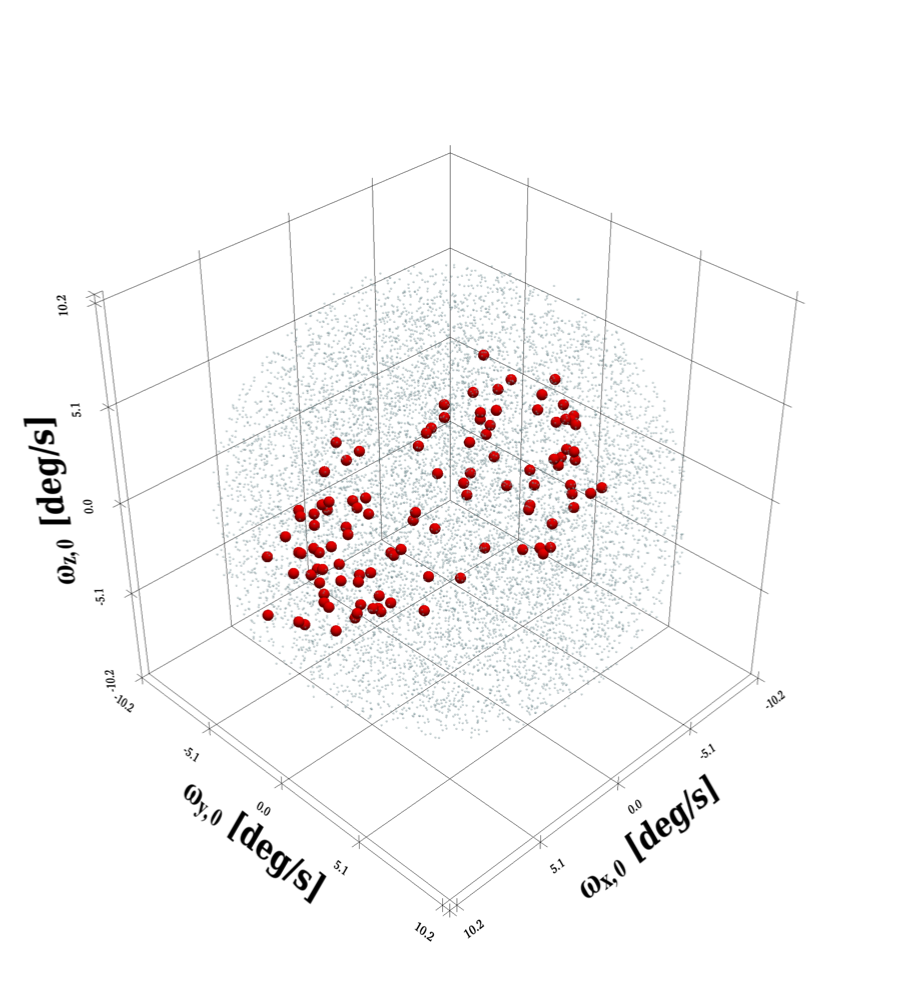
\includegraphics[width=\figmed]{sphx_glr_results_005.png}
%   \caption{Candidate solution angular velocities for the Delta I (Star-37E) rocket body}
%   \label{fig:case2_w}
% \end{figure}

\begin{figure}[H]
  \centering
  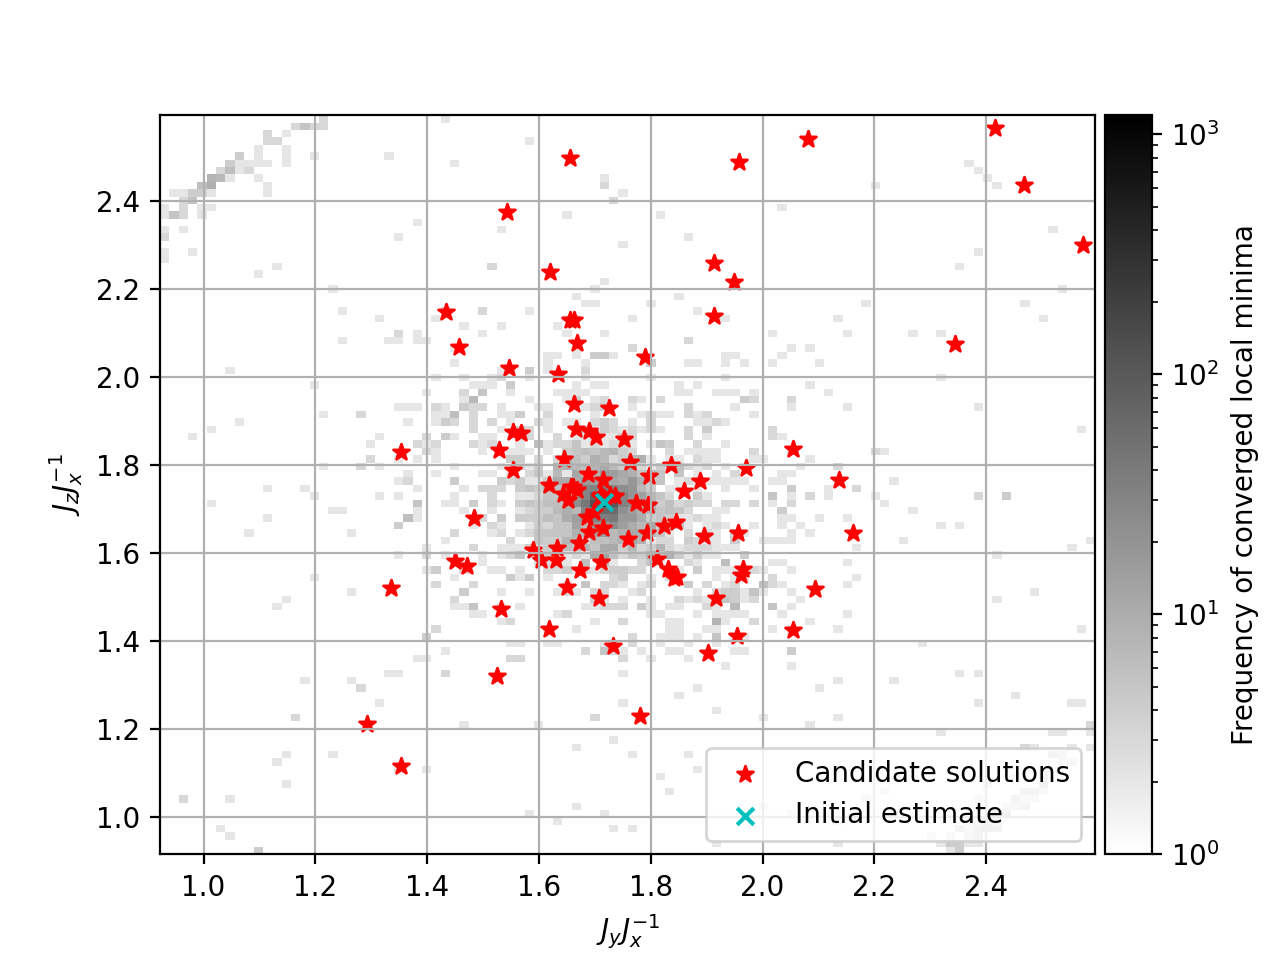
\includegraphics[width=\figsmall]{sphx_glr_results_001_2_00x.png}
  \caption{Candidate solution inertia ratio distribution for the Delta I (Star-37E) rocket body}
  \label{fig:case2_i}
\end{figure}

The candidate solutions identified by the inversion process produce light curves which adequately approximate the measurements, although they do not reach the lowest observed values. This indicates that the true material is more dominated by specular reflections than our assumed coefficients. The candidates show some rough clustering in both orientation and angular velocity space, although they vary significantly in angular velocity magnitude. The inertia tensor solutions display similar variability, although the solutions are spread relatively uniformly from the initial estimate, possibly indicating that the geometry-driven estimate is approximately unbiased. Taken together, these results indicate that the object could be spinning in a number of attitude profiles, although the light curve inversion process has significantly narrowed the search space to small subsets of the original unconstrained eight-dimensional volume. These constraints can be combined with additional light curves, more information about the object's true mass distribution, or reflectivity to further refine the solution set.

\subsection{Case 3: ECHOSTAR II}

In Case 3, we perform attitude inversion on real data observed for a derelict satellite. ECHOSTAR II (COSPAR ID 1996-055A) was a communications satellite on the AS-7000 bus \cite{as7000_astronautix}, shown in Figure \ref{fig:echostar1}. It has an approximate total wingspan of $s = 23.9$ meters, individual solar panel length of $l_p=8.5$ meters, panel width of $w_p=3.1$ meters, and a mass per panel of $m_p = 60$ kilograms \cite{earl2015}. The spacecraft bus is approximately cubic with a side length $w_b=2.3$ meters and a mass of $m_b = 1900$ kilograms \cite{earl2015}.

\begin{figure}[H]
  \centering
  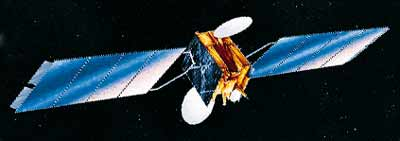
\includegraphics[width=\figbig]{EchoStar-1_image.jpg}
  \caption{ECHOSTAR II artist's rendition \cite{as7000_astronautix}.}
  \label{fig:echostar1}
\end{figure}

\begin{figure}[H]
  \centering
  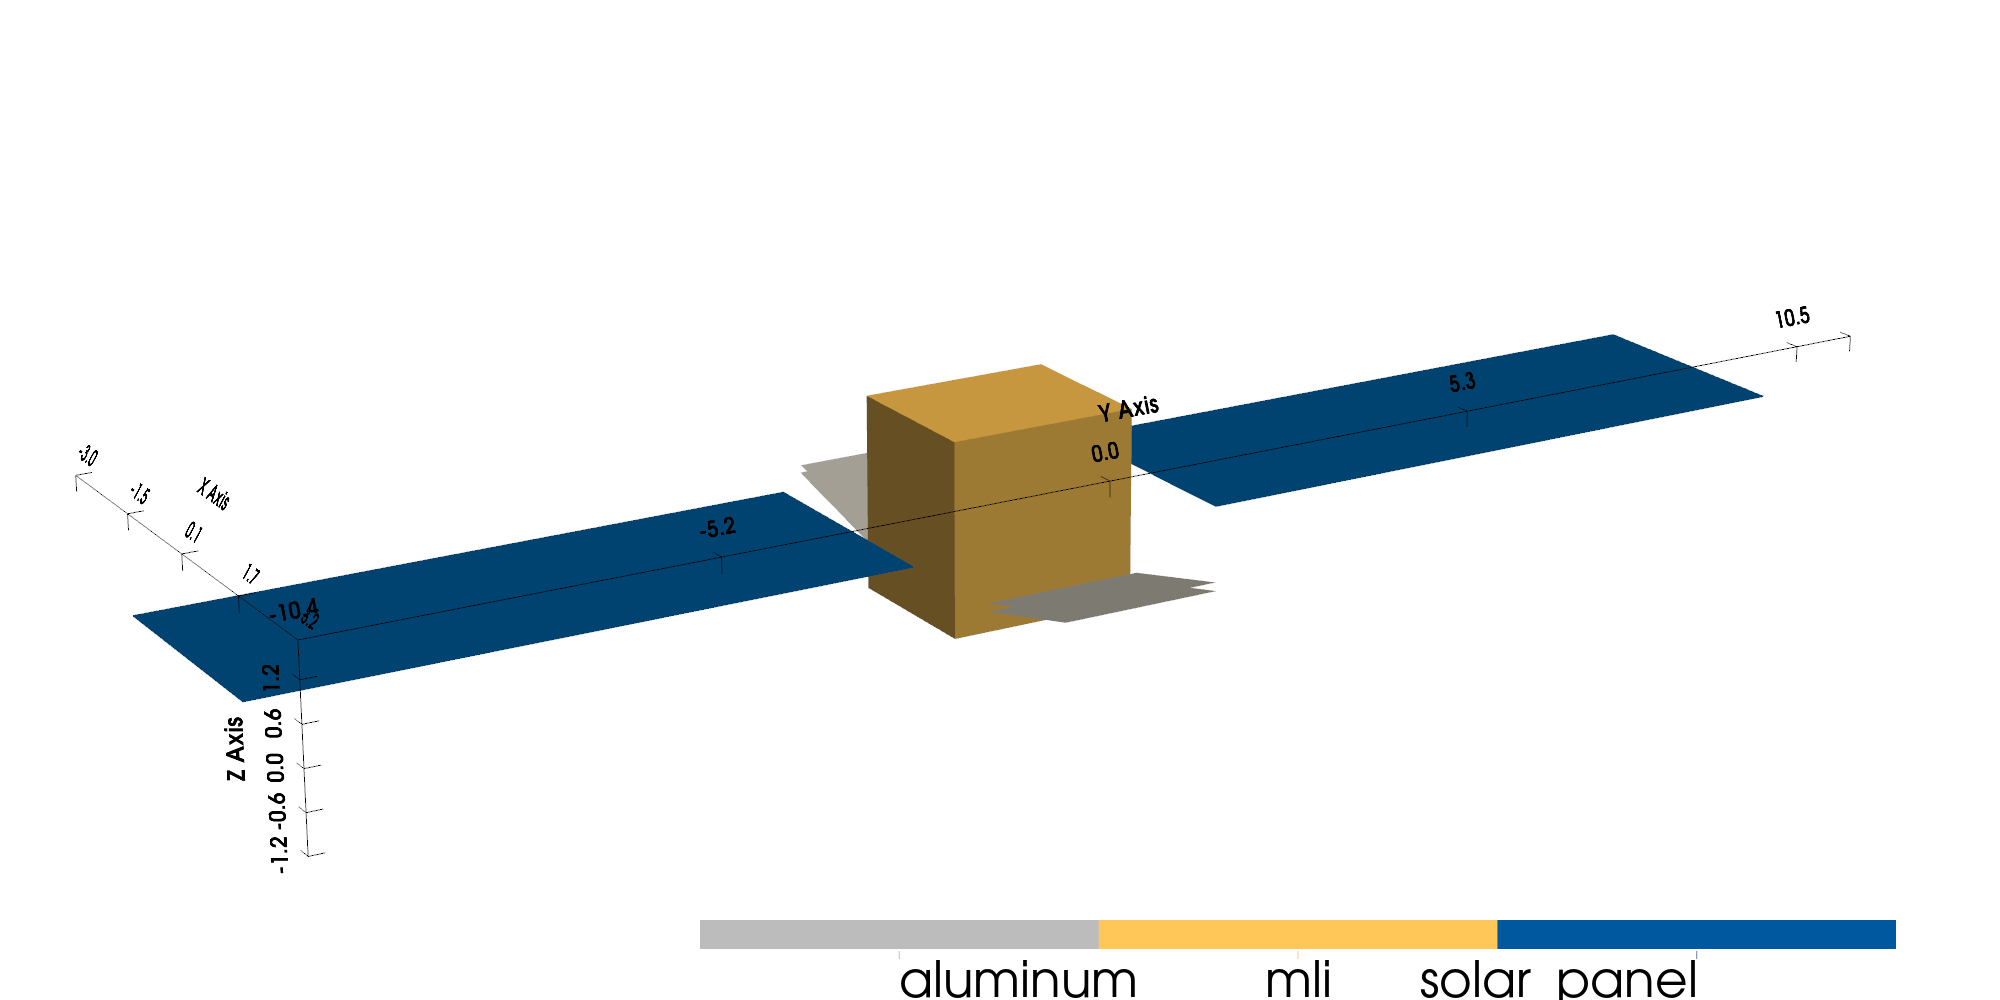
\includegraphics[width=\figbig]{sphx_glr_plot_models_001.png}
  \caption{Simplified ECHOSTAR II box-wing model used for inversion.}
  \label{fig:echostar1_simple}
\end{figure}

The contribution of the bus to the total inertia tensor of ECHOSTAR II is spherically symmetric and given by \cite{satterly1958}:

\begin{align}
 J_\text{bus} &= \frac{1}{6} m_b w_b^2 I_3,
\end{align}

\noindent
assuming that the center of mass (COM) of the bus coincides with the COM of the entire vehicle. By the intermediate axis theorem, the contribution of a panel to the inertia tensor is a function of the displacement of the panel's COM from the vehicle's overall COM $\vctr{r}_p = [ 0, s/2 - l_p/2, 0]^T$:

\begin{equation}
  \begin{split}
 J_\text{pan} = &\frac{m_p}{12} \cdot \text{diag}\left(l_p^2, w_p^2, \left(l_p^2 + w_p^2\right) \right) + \\&m_p \left[ \left( \vctr{r}_p \cdot \vctr{r}_p \right) I_3 - \vctr{r}_p \vctr{r}_p^T \right],
  \end{split}
\end{equation}

\noindent
assuming that the panels have negligible thickness. The overall inertia tensor for ECHOSTAR II is therefore:

\begin{align}
 J_\text{SAT} &= J_\text{bus} + 2J_\text{pan} \\
  &= \text{diag} \left( 9512, 1771, 9609 \right) \: [kg \cdot m^2]
\end{align}

Table \ref{tb:case2_in} summarizes the light curve observations that result in the extracted measurements displayed in Figure \ref{fig:rb_lc_obs}.

\begin{table}[H]
  \centering
  \renewcommand{\arraystretch}{1.3} % Increase row height for better readability
  \caption{ECHOSTAR II observation characteristics}
  \vspace*{6pt}
  \begin{tabular}{@{} l l @{}}
    \toprule
    Variable & Value \\ \midrule
    Target COSPAR ID & 1996-055A \\ \grule
    First obs.\ (UTC) & Feb 26, 2025 04:16:12.279 \\ \grule
    Light curve duration & $19.5$ minutes \\ \grule
    Observations & $456$ ($395$ extracted) \\ \grule
    Obs.\ frequency & $0.388$ Hz \\ \grule
    Integration time & $1$ seconds \\ \brule
  \end{tabular}
  \label{tb:case3_in}
\end{table}

\begin{figure}[H]
  \centering
  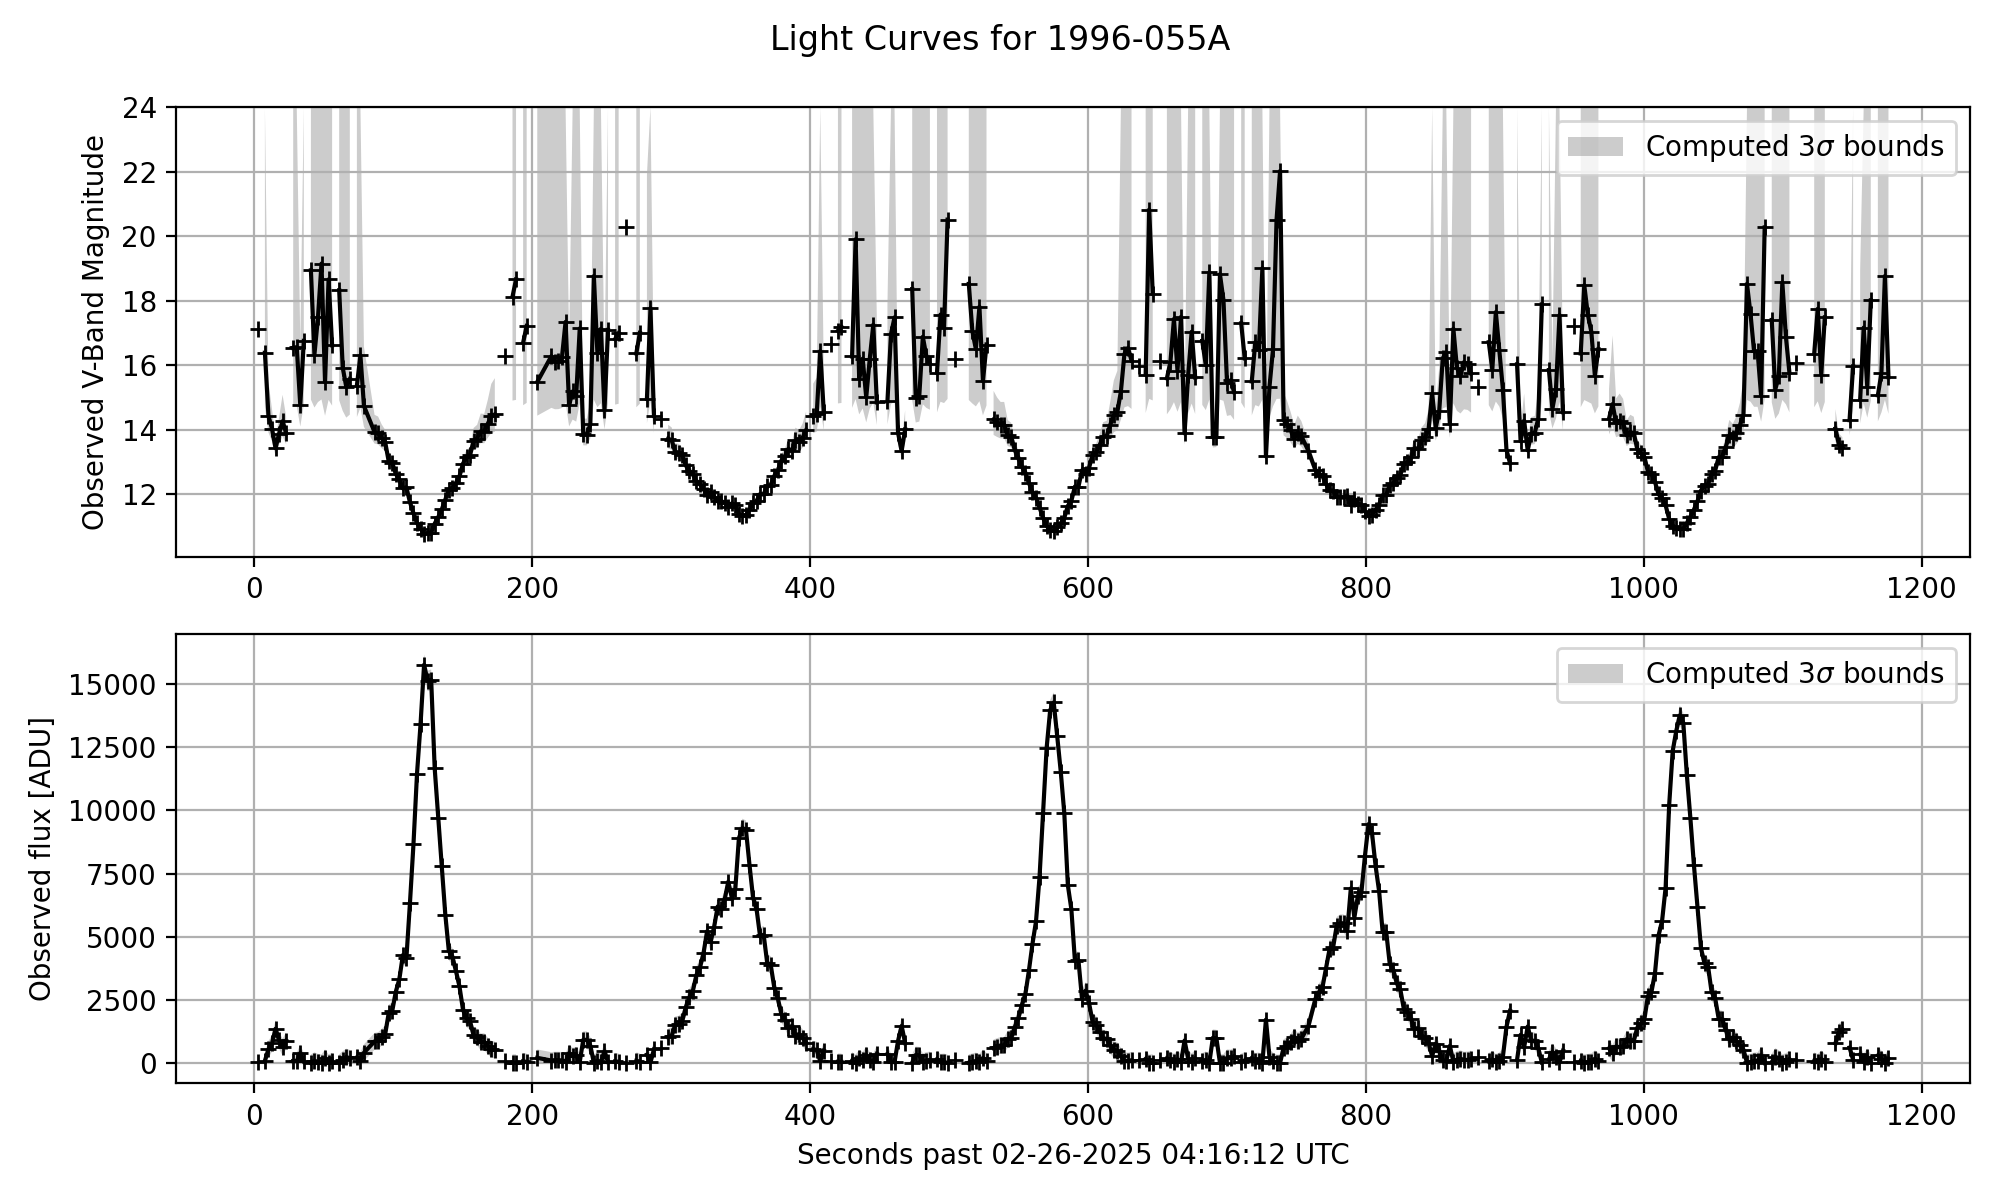
\includegraphics[width=\figbig]{sphx_glr_plot_lcs_002_2_00x.png}
  \caption{Selected light curve for ECHOSTAR II, observed by the Purdue Optical Ground Station}
  \label{fig:sat_lc_obs}
\end{figure}

This light curve is sampled more densely than the Delta I observations, and clearly has significantly more intense specular peaks. Inversion is performed using $n_\text{sample}=10^4$ samples with the material and angular velocity assumptions listed in Table \ref{tb:case3_ass}. Initial state sampling is accomplished identically to Case 2, with a different maximum angular veloity and initial inertia ratios. The candidate solution results are presented in terms of their mean light curves in Figure \ref{fig:case3_s}, orientation MRPs and angular velocities in Figure \ref{fig:case3_pw}, and inertia ratios in Figure \ref{fig:case3_i}. Since the light curve spans three orders of magnitude with a high signal-to-noise ratio, the shape and material mismatch produces specular peaks that are good fits, but are possibly hundreds of standard deviations away from the computed measurement distribution. To combat this, $\ell$ is selected to be much more permissive in selecting candidate solutions compared to previous cases.

\begin{table}[H]
  \centering
  \renewcommand{\arraystretch}{1.3} % Increase row height for better readability
  \caption{ECHOSTAR II inversion assumptions}
  \vspace*{6pt}
  \begin{tabular}{@{} l l @{}}
    \toprule
    Variable & Value \\ \midrule
    Aluminum BRDF & $C_d=0.22$, $C_s=0.4$, $n=5$ \\ \grule
    MLI BRDF & $C_d=0.05$, $C_s=0.24$, $n=20$ \\ \grule
    Solar panel BRDF & $C_d=0.05$, $C_s=0.13$, $n=10$ \\ \grule
    $\norm{\vctr{\omega}}_\text{max}$ & $2.32$ $\text{deg} / \text{s}^{-1}$ \\ \grule
    $\ell$ & $1/1000$ \\ \brule
  \end{tabular}
  \label{tb:case3_ass}
\end{table}

\begin{figure}[H]
  \centering
  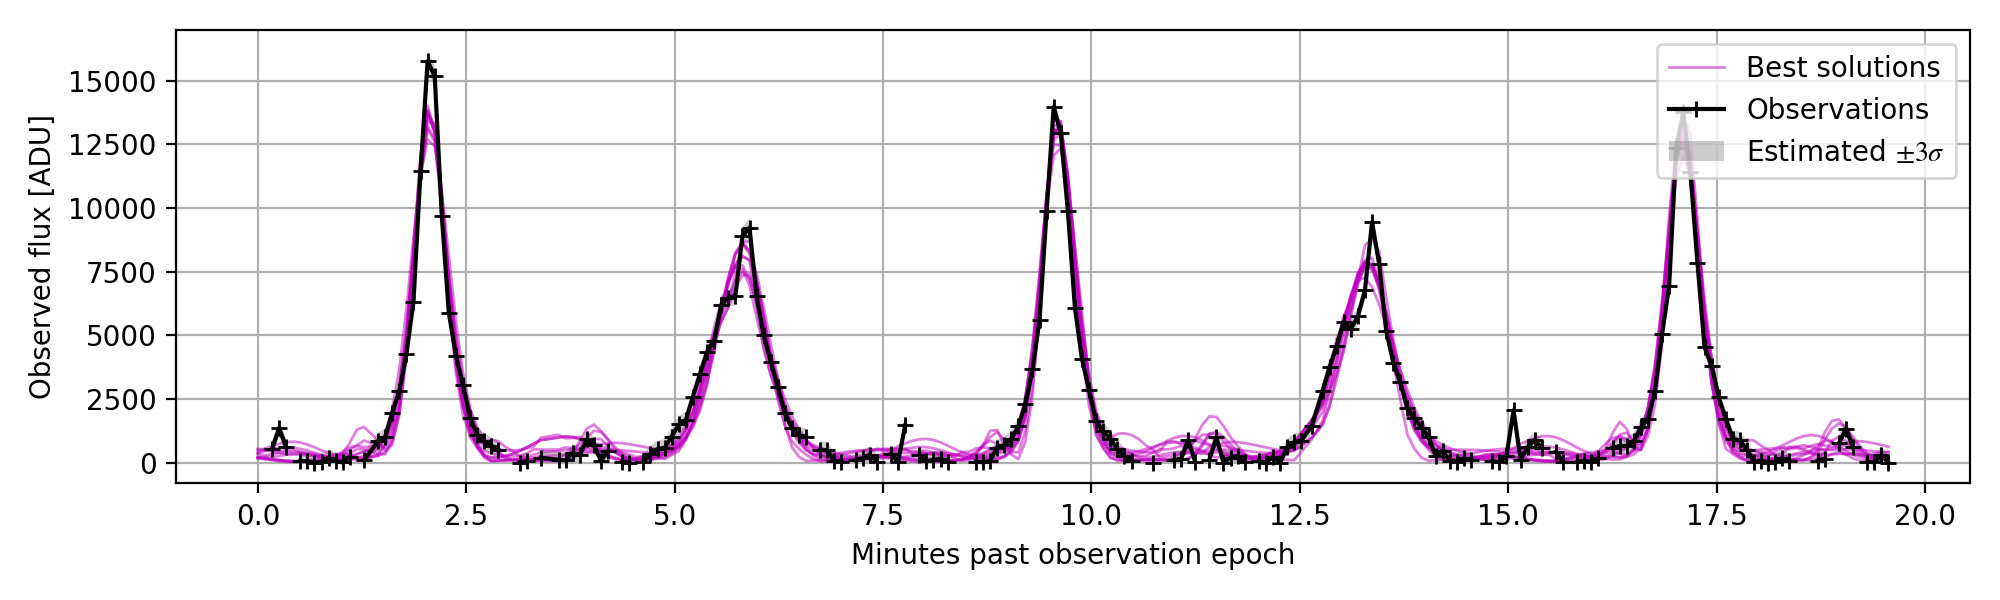
\includegraphics[width=\figbig]{sphx_glr_results_004_2_00x.png}
  \caption{Candidate solution light curves compared to the real measurements in ADU for ECHOSTAR II.}
  \label{fig:case3_s}
\end{figure}

\begin{figure}[H]
  \centering
  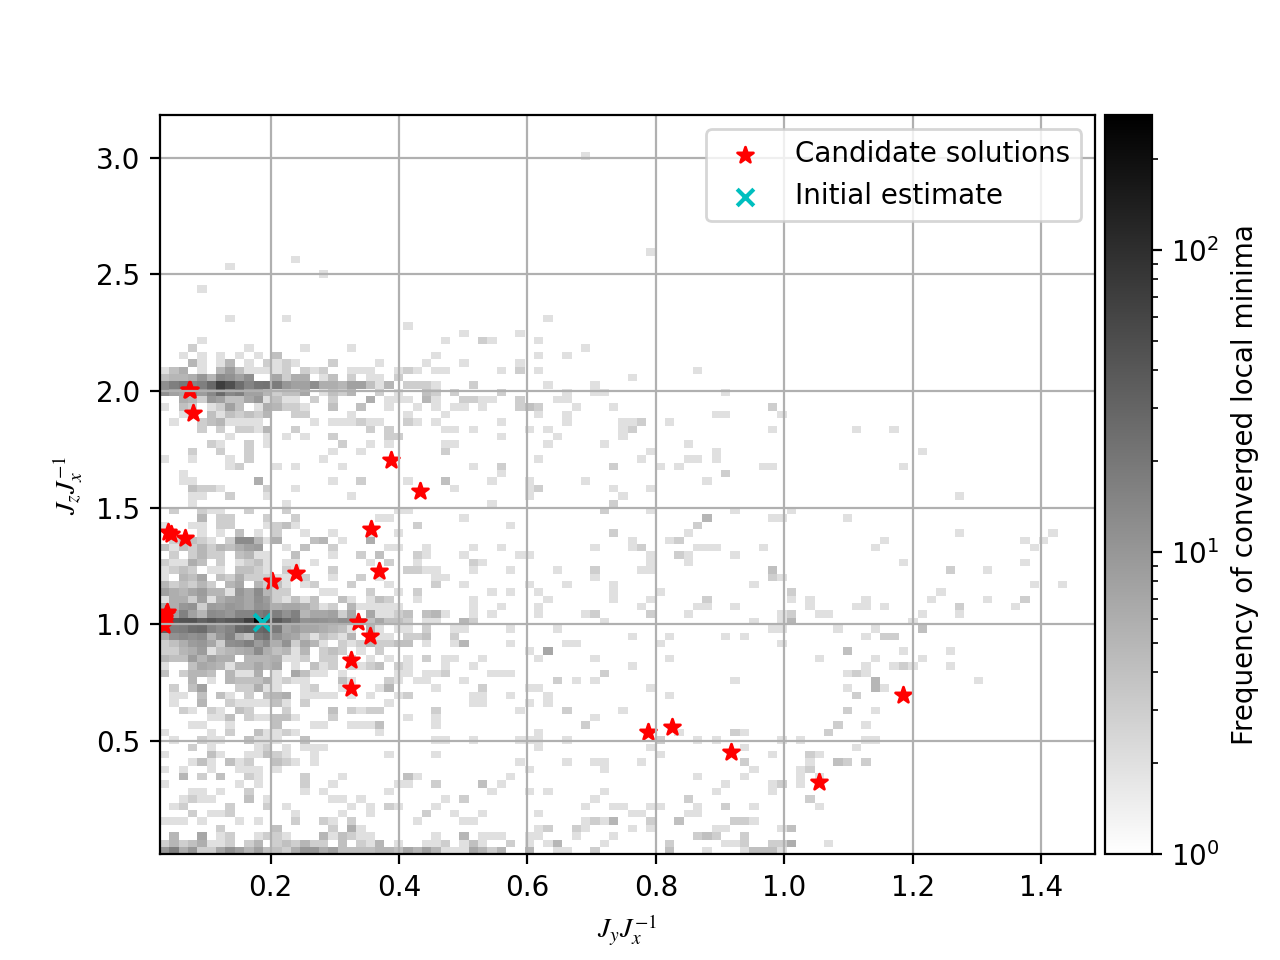
\includegraphics[width=\figsmall]{sphx_glr_results_003_2_00x.png}
  \caption{Candidate solution inertia ratio distribution for ECHOSTAR II with initial estimate in red.}
  \label{fig:case3_i}
\end{figure}

\begin{figure}[H]
  \centering
  \begin{subfigure}[t]{0.23\textwidth}
    \centering
    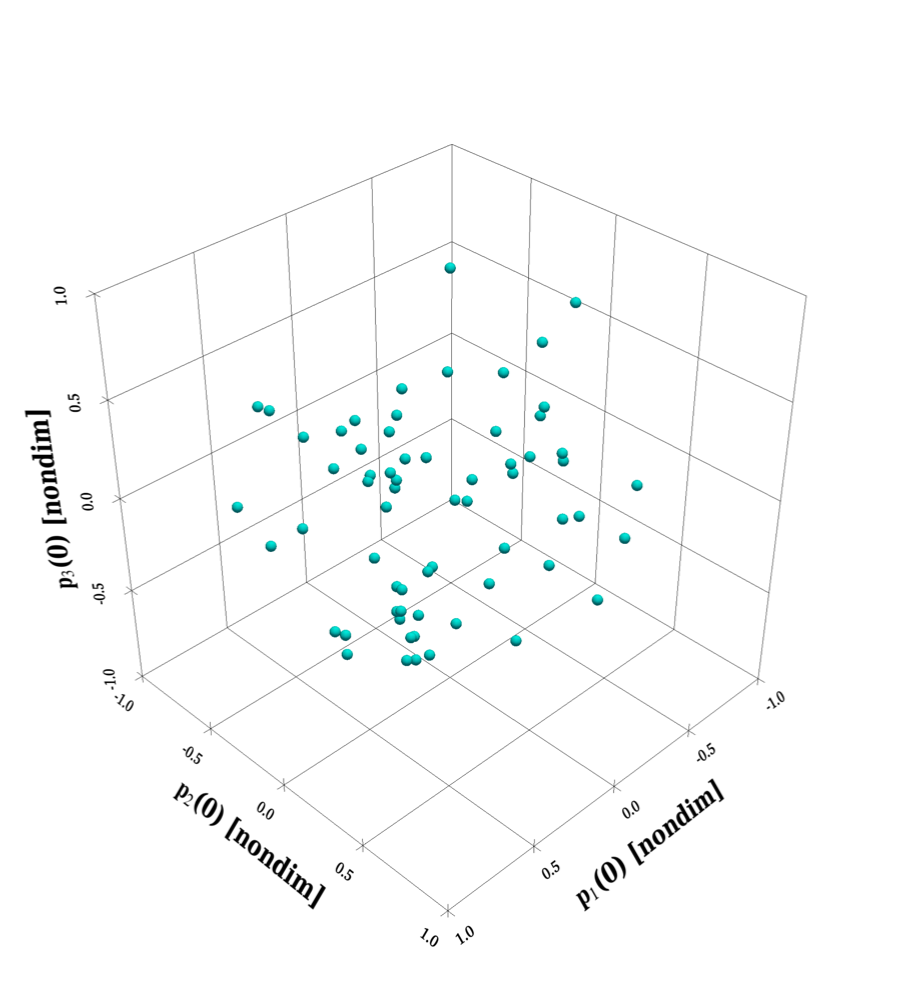
\includegraphics[width=\textwidth]{sphx_glr_results_008.png}
    \caption{}
    \label{fig:case3_pwa}
  \end{subfigure}
  \hfill
  \begin{subfigure}[t]{0.23\textwidth}
    \centering
    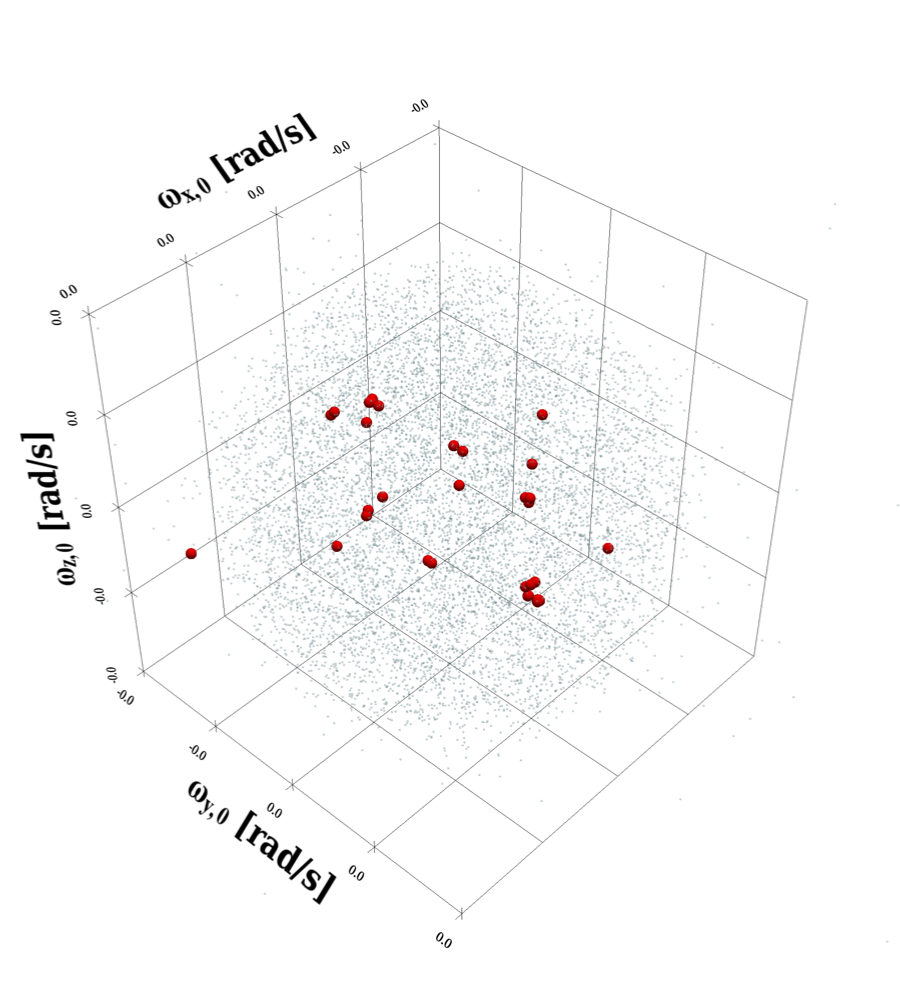
\includegraphics[width=\textwidth]{sphx_glr_results_007.png}
    \caption{}
    \label{fig:case3_pwb}
  \end{subfigure}

  \caption{Candidate solution orientation MRPs (left) and angular velocity vectors (right) for ECHOSTAR II}
  \label{fig:case3_pw}
\end{figure}

% \begin{figure}[H]
%   \centering
%   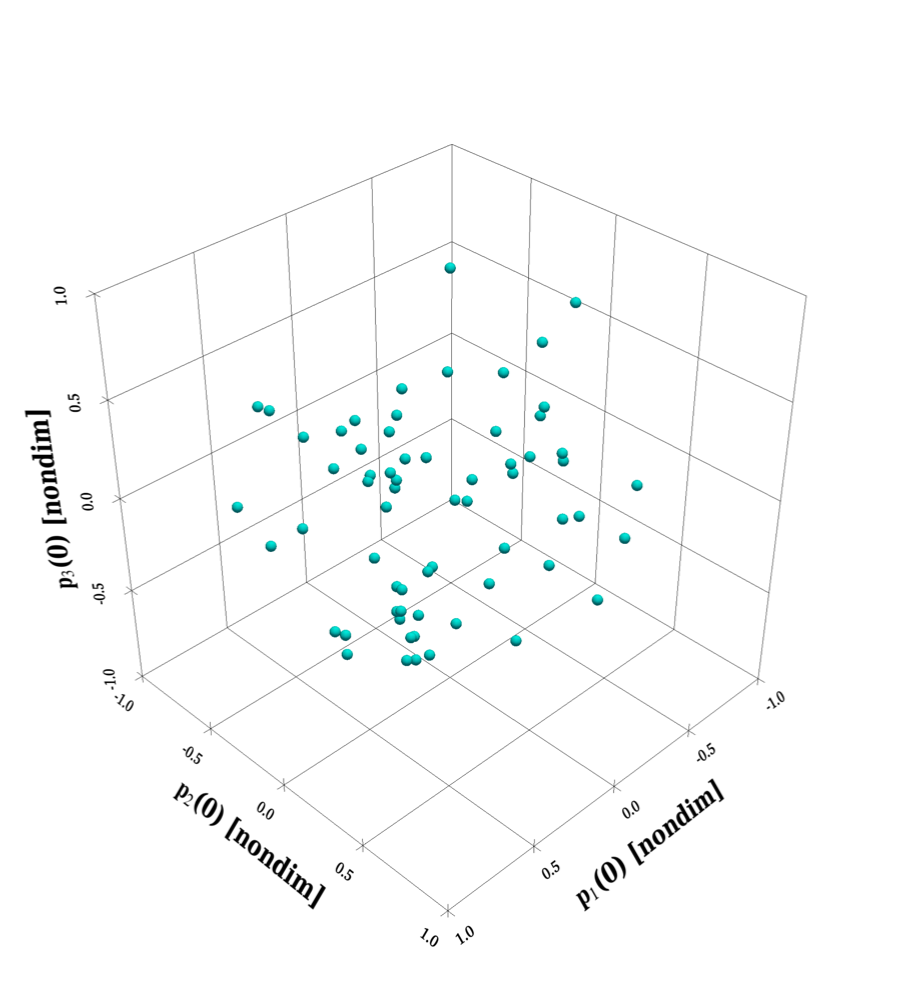
\includegraphics[width=\figmed]{sphx_glr_results_008.png}
%   \caption{Candidate solution orientation MRPs for ECHOSTAR II}
%   \label{fig:case3_p}
% \end{figure}

% \begin{figure}[H]
%   \centering
%   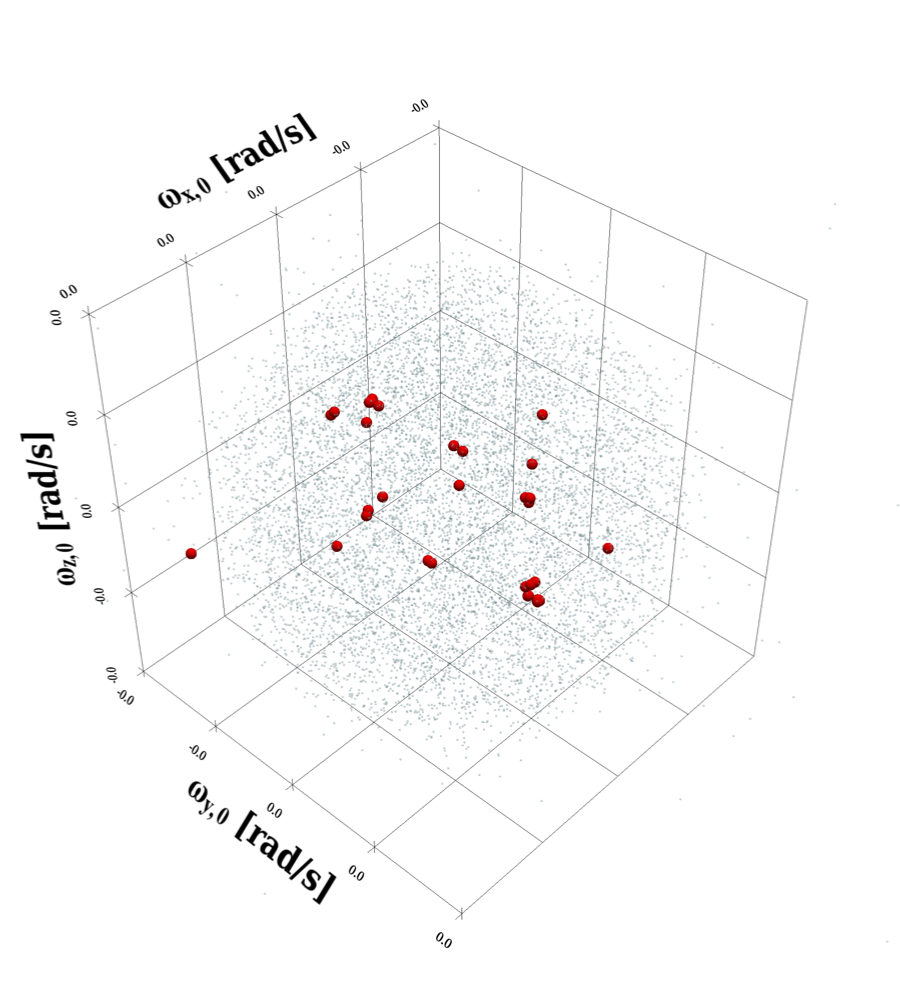
\includegraphics[width=\figmed]{sphx_glr_results_007.png}
%   \caption{Candidate solution angular velocities for ECHOSTAR II}
%   \label{fig:case3_w}
% \end{figure}

The candidate solutions identified by the inversion process are more sparse than those found in either of the previous rocket body cases, with some vague clustering in both angular velocity and orientation space. That said, the candidate light curves fit the data quite well. Notably, the formulation of the negative log-likelihood objective function in Equation \ref{eq:nll_loss} produces the behavior seen in the candidate solutions in Figure \ref{fig:case3_s}, where even the smallest recurrent specular peaks are well-estimated by most solutions. A similar effect -- giving up some of the statistical robustness of our formulation -- can be achieved in an unweighted optimization over the observations in magnitudes. The inertia tensor solutions are dispersed throughout the solution space, with less symmetry than the Delta I solutions. As in the Delta I case, the attitude inversion solver has successfully constrained the search space for later optimization as more data about the mass and reflectivity of the object becomes available to continue refining any of these candidates.

\section{Conclusion}

Attitude information is critical for many tasks informing space situational awareness. Orientation and angular velocity data aids high-fidelity orbit propagation, mission recovery efforts, and object selection for active debris removal. Obtaining attitude information is often difficult, especially for passive debris objects. Due to atmospheric distortion and diffraction-limited optics, ground-based telescopes can only determine a total brightness received from a space object. If a shape model is known, the light curve -- a sequence of these brightness measurements -- is one tool for attitude estimation. We presented an approach for solving this highly nonlinear and non-convex optimization problem with a gradient-based multi-start method. We presented attitude inversion results for one case with synthetic data and two cases with real observations. Unlike other approaches, our method successfully identifies the numerous ambiguous solutions families -- originating from symmetries in the observation geometry and the object shape -- which can produce the same observations. These disparate candidate solutions can serve as starting points for more detailed exploration as additional light curves or further object shape information is obtained.

\section{Global TODO list}

\begin{itemize}
  % \item Add the constant term back into the objective function (in text and code) so we can start treating it as a real likelihood, useful for the future
  \item Mention the unknown solar panel rotation angle for ECHOSTAR
  \item make a table of execution times
  % \item Update perspective on some the case 1a angular velocity plot
  % \item Update $n_\text{sample}$ values everywhere to reflect the scripts
  % \item Update $\omega$ sampling scheme to go from $0.5-2$ as reflected in scripts
  % \item Re-run all cases to ensure that values are up to date with recent changes, update where those statistics are reported in the text
  \item Try to get rid of big gaps where possible
  % \item Reformat tables so they're attractive to look at
\end{itemize}

\section*{Acknowledgments}

This work was partially supported by a National Defense Science and Engineering Graduate Fellowship.

\section*{Appendix}

\begin{table}[H]
  \centering
  \renewcommand{\arraystretch}{1.3} % Increase row height for better readability
  \caption{Telescope information for synthetic and real data observations}
  \vspace*{6pt}
  \begin{tabular}{@{} l l @{}}
    \toprule
    Variable & Value \\ \midrule
    CCD sensor & KAF-16803 \\ \grule
    Aperture area ($A_\circ$) & $0.076$ m$^2$ \\ \grule
    Observer location & $32.900^\circ$ N, $-105.533^\circ$ W \\ \grule
    Observer altitude & $2.24$ km above MSL \\ \grule
    Read noise ($\sigma_\text{read}$) & $9$ ADU/pixel \\ \grule
    Dark current rate ($\lambda_\text{dark}$) & $0.01$ ADU/pixel/s \\ \grule
    Flat field strength ($f_k$) & $0.01$ (dimensionless) \\ \grule
    Gain ($g$) & $5.1$ e$^-$/ADU \\ \brule
  \end{tabular}
  \label{tb:tele_info}
\end{table}

\begin{table}[H]
  \centering
  \renewcommand{\arraystretch}{1.3} % Increase row height for better readability
  \caption{BFGS solver configuration for all results cases}
  \vspace*{6pt}
  \begin{tabular}{@{} l l @{}}
    \toprule
    Variable & Value \\ \midrule
    Maximum function evaluations & $1000$ \\ \grule
    Maximum iterations & $100$ \\ \grule
    Finite difference step size & $1 \cdot 10^{-5}$ \\ \grule
    Gradient $\infty$-norm tolerance & $1 \cdot 10^{-5}$ \\ \brule
  \end{tabular}
  \label{tb:bfgs_info}
\end{table}


\bibliography{cache/refs.bib}
\end{document}

